\expandafter\def\csname CTEX@spaceChar\endcsname{\hspace{1em}}
\documentclass[UTF8, pdftex, notypeinfo, hyperref]{CASthesis}
\usepackage{indentfirst} % 首行缩进
\usepackage{amssymb,bm,mathrsfs,bbm,amscd}
\usepackage{hepunits}
\usepackage{caption,subcaption}
\usepackage{multirow}
\usepackage[hidelinks,bookmarksdepth=4]{hyperref}
\usepackage{xcolor}
\usepackage{listings}
\usepackage{lineno}
\usepackage{pdfpages}
\usepackage[draft]{todonotes}
\usepackage{geometry}
\geometry{left=3.17cm,right=3.17cm,top=2.54cm,bottom=2.54cm}

\setlength{\marginparwidth}{0.5cm}
% 设置图形文件的搜索路径
\graphicspath{{chapter/}{figures/}}

\usepackage{graphicx}          %设置eps转化为pdf
\usepackage{epstopdf}          %插图使用的是eps,生成的是pdf的插图

\usepackage{verbatim}          %可以使用命令注释掉大量的文字

%\usepackage{subfig} 
%\usepackage{subfigure}         %subfigure

% 取消链接的颜色(黑白打印时)
%\hypersetup{
%    colorlinks=false,
%}

% 小节标题靠左对齐
\CTEXsetup[format+={\flushleft}]{section}

\begin{document}


%%%%%%%%%%%%%%%%%%%%%%%%%%%%%%
%% 封面部分
%%%%%%%%%%%%%%%%%%%%%%%%%%%%%%

  % 中文封面内容
  \confidential{}
  \title{BESIII多气隙电阻板室飞行时间探测器刻度方法的研究}
  \author{郭迎晓}
  \advisor{孙胜森~研究员}
  \advisorinstitute{中国科学院高能物理研究所}
  \chinesedegree{硕士}
  \majordegree{工程硕士}
  \major{计算机技术}
  \submitdate{2017~年~6~月}
  \institute{中国科学院高能物理研究所}

  % 英文封面内容
  \englishtitle{Study of calibration of the Multigap-Resistive Plate Chamber as Time of Flight Detector in BESIII experiment}
  \englishauthor{Yingxiao Guo}
  \englishadvisor{Prof. shengsen sun}
  \englishinstitute{Institute of High Energy Physics}
  \englishdegree{Master}
  \englishmajordegree{Engineering}
  \englishdate{June, 2016}

  % 封面
  %\maketitle

  % 英文封面
  %\makeenglishtitle

  \includepdfmerge{cover.pdf, 1-4}
%  \includepdfmerge{coversecret.pdf, 1-4}
  \includepdfmerge{statement.pdf}                 %直接插入中文,英文的封面

%%%%%%%%%%%%%%%%%%%%%%%%%%%%%%
%% 前言部分
%%%%%%%%%%%%%%%%%%%%%%%%%%%%%%
\frontmatter

  \pagenumbering{Roman}                  %设置页脚为大写的Roman字符
  %\setcounter{page}{0}
 

  % 摘要
  % !TeX root = ../main.tex
% !TEX root = ../main.tex
% -*- root: ../main.tex -*-
% -*- program: pdflatex -*-

\begin{abstract}
北京谱仪(BESIII)的物理目标是对~$\tau$-粲(c)物理进行高精度的实验测量并寻找新物理。在较大的动量范围内很好地鉴别区分各种带电粒子是~BESIII~探测器设计的要求。BESIII~探测器的粒子鉴别系统主要由主漂移室(MDC)的~dE/dx~和飞行时间探测器(TOF)组成。飞行时间探测器的主要物理目标是粒子鉴别(PID),粒子鉴别能力的大小由相同动量不同种类粒子的飞行时间差和时间分辨决定。升级改造前的端盖飞行时间探测器采用塑料闪烁体直接耦合光电倍增管的方案,对于~$\pi$~介子,时间分辨达到~138~ps,已经不能满足~BESIII~实验高精度测量的需要。2015~年~10~月,BESIII~实验完成了端盖~TOF~的升级改造,用时间分辨性能更好的多气隙电阻性板室(MRPC)替代了原来的闪烁体,新的探测器参与了~2015-2016~运行取数。对~MRPC~端盖~TOF~离线数据刻度算法进行研究,并开发相关的软件,通过消除原始测量时间随粒子击中位置和过阈时间(Time over Threshold,TOT)的游动,进一步提高粒子鉴别能力,对实现~BESIII~高精度测量的物理目标是十分重要和不可或缺的。

国际上,相对论重离子对撞机(RHIC)上的~STAR~实验和大型强子对撞机(LHC)上的~ALICE~实验都采用了~MRPC~作为飞行时间探测器,结合他们各自的特点,分别采用多次样条插值和多项式拟合方法进行探测器刻度。

MRPC~端盖~TOF~的离线刻度算法软件基于~BESIII~离线数据处理和分析软件平台(BOSS)。利用~BESIII~实验获得的真实数据,通过在线事例分类得到~Bhabha~事例做为刻度样本,对刻度算法进行了研究。研究对测量时间随带电粒子击中读出条位置,过阈时间的变化关系,以及他们之间的关联进行了分析。论文首先利用多次样条插值方法构造刻度算法,对原始测量时间随过阈时间的复杂的依赖关系进行了刻度,研究发现由于信号反射的存在,这种刻度方法的效果并不理想。通过对过阈时间的击中位置依赖关系的分析,揭示了信号在读出条内的反射造成~TOT~多峰的形成机制。然后在构造刻度公式方法中,首先对击中位置进行了刻度,这个过程同时也消除了过阈时间对击中位置的依赖,然后再对时间-幅度的关系进行刻度,收到了良好的效果,单条时间分辨达到~53.5~ps。论文还对刻度公式的适用性问题,以及刻度算法中过阈时间和击中位置的关联性进行了讨论。最后,论文介绍了离线刻度算法软件的实现。

利用~BESIII~获取的~Bhabha~事例样本,对升级改造后的~MRPC~端盖~TOF~的离线数据刻度算法进行了研究,确定了刻度的流程,构造了合理的刻度公式,完成了相关软件的开发。离线刻度的结果优于探测器硬件设计指标,新的刻度算法将会对~BESIII~获得高精度的测量结果产生积极的促进作用。

\keywords{离线刻度,多次样条插值,多气隙电阻性板室,飞行时间探测器,北京谱仪}
\end{abstract}

\begin{englishabstract}
%北京谱仪(BESIII)的物理目标是对tau-粲(c)物理进行高精度的实验测量并寻找新
Physics goal of BESIII are the tau-c physics in experimental measurement with high precision and searching new physics.
%物理。在较大的动量范围内很好地鉴别区分各种带电粒子是BESIII探测器设计的要求。
In a large range of momentum, it is required to identify all species of charged tracks weel in design of BESIII detector.
%BESIII探测器的粒子鉴别系统主要由主漂移室(MDC)的dE/dx和飞行时间探测器
The particle identification system of BESIII detector consists of Main Drift Chamber(MDC) which is providing the measurement of dE/dx and Time of Flight Detector(TOF).
%(TOF)组成。飞行时间探测器的主要物理目标是粒子鉴别(PID),粒子鉴别能力的大小由相同动量不同种类粒子的飞行时间差和时间分辨决定。升级改造前的端盖飞行时间探
The main physical goal of TOF is to implement the Particle Identification(PID), and PID capability is determined by the different values of the time of flight for different species of particles with the same momentum and the time resolution.
%测器采用塑料闪烁体直接耦合光电倍增管的方案,对于pi介子,时间分辨达到138ps,已经不能满足BESIII实验高精度测量的需%要。2015%年10月,BESIII实验完成了端盖TOF的升级改造,用时间分辨性能更好的多气隙电阻性板室(MRPC)替代了原来的闪烁体,新的%探测器参与了2015~2016运行取数。对MRPC端盖TOF离线数据刻度算法进行研
Before the upgrade, the endcap TOF adopted the project using plastic scintillator coupled with photomultiplier tubes(PMT) directly, and the time resolution is 138ps for pions. However, it couldnot satisfied the requirement of the high precision of BESIII experimental measurement. In October, 2015, the upgraded endcap TOF have been completed in BESIII experiment. And the new endcap TOF based on MRPC which has a better time resolution to substitute plastic scintillator. This new detector technology has been participate the physical data taking in the period of the year 2015 to 2016.
%究,通过消除原始测量时间随粒子击中位置和过阈时间(Time over Threshold,TOT)的游动,进一步提高粒子鉴别能力,对实现%BESIII高精度测量的物理目标是十分重要和不可或缺的。
And the study of the offline data calibration algorithm and develop the relevant software for MRPC endcap TOF is eliminate the original measurement of time with the dependence of the particle hit position and the time-walk of Time over Threshold(TOT), this study further improve the capability of PID, and is important and indispensable to reach the physical goal of high precision measurement at BESIII. 

%国际上,相对论重离子对撞机(RHIC)上的STAR实验和大型强子对撞机(LHC)上的ALICE实验都采用了MRPC作为飞行时间探测器,结合%他们各自的特点,分别采用多次样条插值和多项式拟合方法进行探测器刻度。
Both the STAR experiment in RHIC and the ALICE experiment in LHC used MRPC as their TOF detector. And considering their own characters, the offline date are calibrated using spline-fit method and polynomial fitting method.

%MRPC端盖TOF的离线刻度算法基于BESIII离线数据处理和分析软件平台(BOSS)。利用BESIII实验获得的真实数据,通过在线事例分类得%到Bhabha事例做为刻度样本,对刻度算法进行了研究。
The offline data calibration algorithm of MRPC endcap TOF is based on BESIII offline data processing and analysis software(BOSS). The calibration data sample is Bhabha events of real data which is selected.
%研究对测量时间随带电粒子击中读出条位置,过阈时间的变化关系,以及他们之间的关联进行了分析。论文首先利用多次样条插值方法构造刻度算法,对原始测量时间随过阈时间的复杂的依赖关系进行了刻度,研究发现由于信号反射的存在,这种刻度方法的效果并不理想。通过对过阈时间的击中位置依赖关系的分析,揭示了信号在读出条内的反射造成TOT多峰的形成机制。在构造刻度公式方法中,首先对击中位置进行了刻度,这个过程同时也消除了过阈时间对击中位置的依赖,然后再对时间-幅度的关系进行刻度,收到了良好的效果,时间分辨达到**ps。论文还对刻度公式的适用性问题,以及刻度算法中过阈时间和击中位置的关联性进行了讨论。
This study analyzed the alternative relations of the measurement time changes with hitted positions and TOT of signal, and also  analyzed their the corelation between these variables. This paper first constructed a calibration algorithm by spline-fit method, and calibrated the original measurement time with the complex change of TOT. The Spline fit method is not ideal due to the presence of signal reflections found by studies. Then, the dependency of the hit position of TOT has been investigated, it explained how the reflection of the signal within the readout strips causes the formation mechanism of the TOT multimodal. In the construction of the calibration formula, the hit position has been performed first, at the same time, the hit position dependency of TOT can be eliminated. And then, correct time versus TOT, it has good effect, the time resolution reached 53.5ps in one strip. The applicability of these calibration formula and the relevance between TOT and hit position in calibration algorithm are also discussed in this paper.Finally, the paper introduces the implementation of the software of the offline calibration algorithm.    

%利用BESIII获取的Bhabha事例样本,对升级改造后的MRPC端盖TOF的离线数据刻度算法进行了研究,确定了刻度的流程,构造了合理的刻度公式。离线刻度的结果优于探测器硬件设计指标,新的刻度算法将会对BESIII获得高精度的测量结果产生积极的促进作用。
Using the Bhabha samples collected from BESIII, the offline data calibration algorithm of the upgraded MRPC endcap TOF detector has been studied, determined the process of calibration, constructed reasonable calibration formula and complete the development of relevant software. The result of offline data calibration is better than design target of the detector hardware, and the new calibration algorithm will play a positive role in getting the high precision measurement results at BESIII.


\englishkeywords{Offline Data Calibration,Spline Fit,Multi-gap Resistive Plate Chamber, Time of Flight Counter,BESIII}

\end{englishabstract}


  % 目录
  \tableofcontents
  % 表格目录
  \listoftables
  % 插图目录
  \listoffigures


%%%%%%%%%%%%%%%%%%%%%%%%%%%%%%
%% 正文部分
%%%%%%%%%%%%%%%%%%%%%%%%%%%%%%
\mainmatter

  \pagestyle{fancy} % 选用 fancy style
  \fancyhf{}   %注释掉之前设置的页眉页脚格式
  \fancyhead[CE]{\small \leftmark}
  \fancyhead[CO]{\small \rightmark}
  \fancyfoot[LE,RO]{\small ~\thepage~}

  % !TeX root = ../main.tex
% !TEX root = ../main.tex
% -*- root: ../main.tex -*-
% -*- program: pdflatex -*-
\chapter{前言}

\section{粒子物理学}

物质是由什么组成的?这是人们研究自然界的普遍规律时关心的问题。在《庄子.天下篇》中,庄子有“一尺之捶,日取其半,万世不竭”的观点。说的是一尺长的捶子,今天取它一半。明天再取它一半的一半,如此取下去,一万世也取不完。这是古代中国的辩证思想,认为物质的组成是没有极限的。中国夏朝时的“五行学说”认为物质是有金、木、水、火、土组成。古希腊也有物质有水、火、土和空气等基本元素组成的观点,Democritus~认为万物由大小不同、质量不同、有不可入性的原子组成,原子是“不可再分”的。十九世纪初英国的科学家道尔顿提出原子理论。认为,物质世界的最小单位是原子,原子是单一的,独立的,不可被分割的,在化学变化中保持着稳定的状态,同类原子的属性也是一致的。这是真正带有近代性质的原子论。十九世纪,自然学科创立并蓬勃发展,物理学、化学等学科相继诞生,通过实验对物质的研究,提出物质都是有分子组成的,不同分子性质的不同导致物质的物理和化学性质的不同。分子是由原子组成的。门捷列夫的元素周期表则给出了物质是由~110~多种的元素组成的。二十世纪物理学蓬勃发展,量子力学和相对论相继建立并发展起来,实验上各类粒子相继被发现。例如~1897~年汤普逊发现电子;~1901~年普朗克提出光量子假说,~1905~年爱因斯坦利用光量子假说成功解释了光电效应;~1911~年卢瑟福提出原子核式结构,并于~1919~年利用~$\alpha$~粒子轰击靶原子发现了质子;~1932~年查德威克在人工核裂变实验中发现了中子;~1932~年在宇宙线实验中发现了正电子,这是人类发现的第一个反粒子;~1937~年发现~$\mu$~子;~1947~年发现~$\pi$~介子;~1950~年发现~$K$~介子,~$\Lambda$~,~$\Sigma$~;~1955~年发现反质子;~1956~年发现反中子;~1974~年发现~$J/\Psi$~介子,证实了粲(c)夸克的存在;~1975~年发现~$\tau$~轻子;~1983~年发现传递弱相互作用的玻色子:~$W^{\pm}$~和~$Z^{0}$~;~1995~年发现顶夸克(top);~2012~年发现标准模型的最后一个基本粒子希格斯(~Higgs~)~\cite{ATLAS:2012}\cite{CMS:2012}。大学的量子力学和原子核物理课程介绍了原子是由原子核和电子组成的,而原子核是由质子和中子组成的。基本粒子的相继发现,促进了粒子物理学的诞生和发展。粒子物理学认为组成原子核的质子和中子是由夸克组成的。~\cite{2014lv}

粒子物理学是研究基本粒子的性质、运动、相互作用、相互转化的规律的学科,是物理学的基础学科,也是物理学研究的最前沿学科~\cite{zhangns2015}~\cite{duds2015}。

自然界存在的四种基本相互作用分别是:引力相互作用,电磁相互作用,强相互作用,弱相互作用。它们的相互作用特点的比较如表~\ref{tbl:interaction}~。其中强相互作用和弱相互作用是短程力,电磁相互作用和引力作用都是长程力。

\begin{table}[h]
    \centering
    \caption{\label{tbl:interaction} 四种基本相互作用性质的比较}
    \footnotesize
    \begin{tabular}{lccccc}
        \hline
        相互作用& 强度& 力程& 媒介子& 参与作用粒子& 束缚态 \\
        \hline
        强作用& 1& $10^{-15}$m& 胶子& 夸克,胶子& 强子 \\
        电磁作用& 1/137& $F \propto 1/r^{2}$& 光子& 带电粒子& 原子 \\
        弱作用& $10^{-5}$& $<10^{-17}$m& $W^{\pm}$,$Z^{0}$& 费米子& 无 \\
        引力& $10^{-39}$&  $F \propto 1/r^{2}$& 引力子?& 所有粒子& 太阳系等\\
        \hline
    \end{tabular}
\end{table}



标准模型~(Standard Model, SM)~是一套目前描述强相互作用~(strong interaction)、弱相互作用~(weak interaction)~和电磁相互作用~(electromagnetic interaction)~这三种基本相互作用以及基本粒子最成功的理论~\cite{duds2015}~\cite{S.Weinberg:1967}。
图~\ref{fig:standard_model_particle}~是基本粒子的示意图。
\begin{figure}[!h]
  \centering
  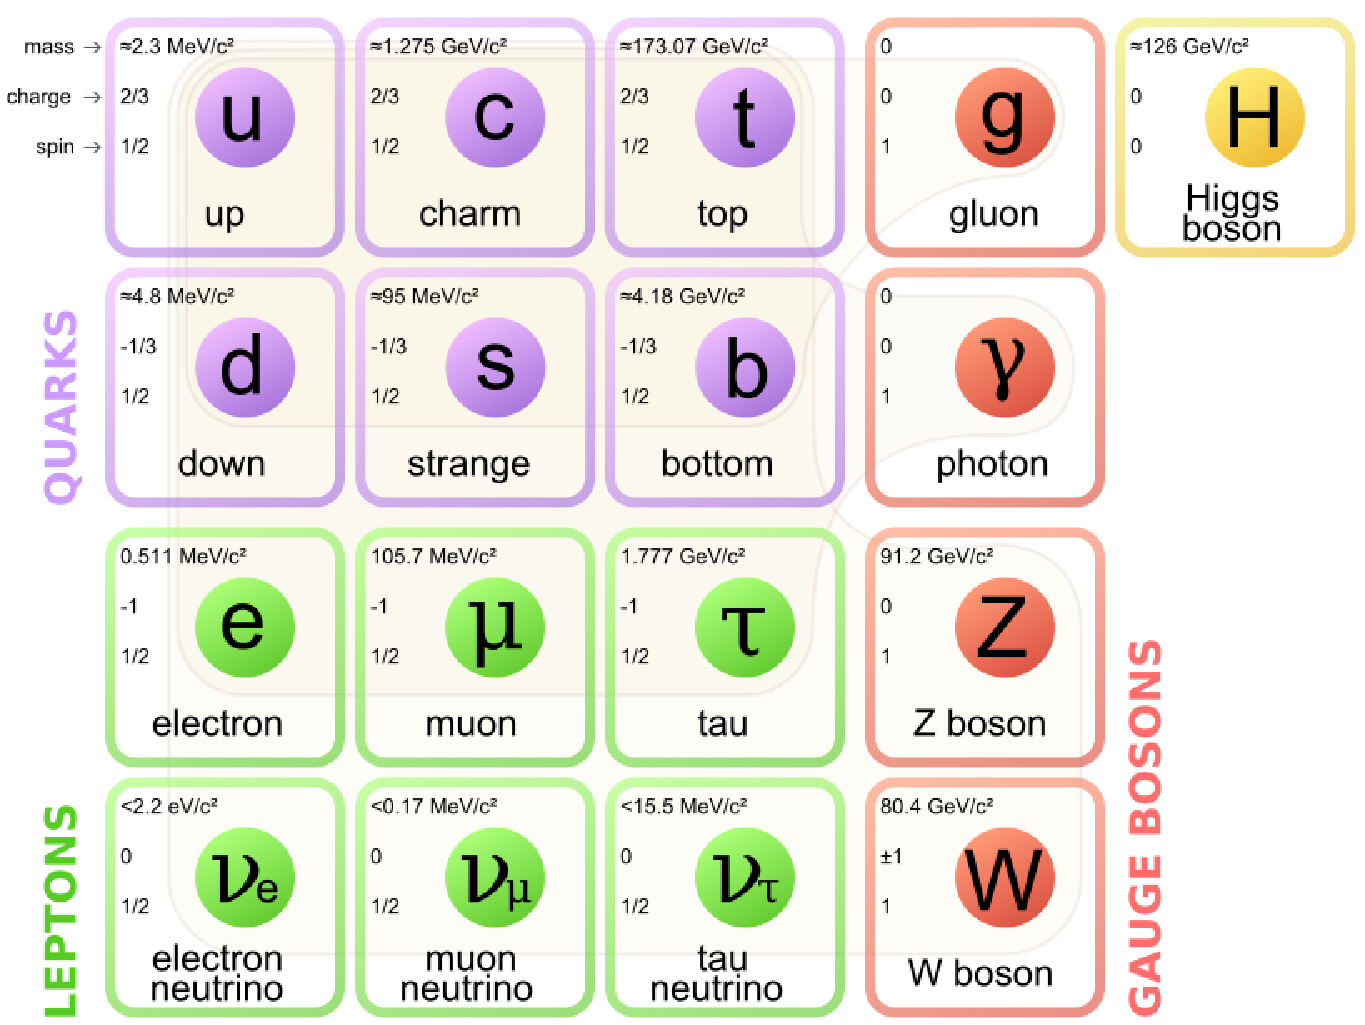
\includegraphics[width=10cm]{chap0/Standard_Model_of_Elementary_Particles.pdf}
  \caption{标准模型中的基本粒子}
  \label{fig:standard_model_particle}
\end{figure}

粒子物理学是一门实验科学。宇宙线,高能物理加速器和粒子探测器是高能物理实验的主要手段~\cite{tangxw1982}~\cite{xukz1981}~\cite{xieyg2003}\cite{xuefj2003}。研究越深层次的物质结构需要越精细的探针:即更高能量的入射粒子。高能加速器具有高能量,高亮度的特点,可控制产生实验所需要的高能粒子束流。

加速器物理实验利用粒子加速器将带电粒子的能量提高到一定状态,通过对撞或者打靶让高能粒子之间(对撞机实验)或者高能粒子和其他物质之间(固定靶实验)发生相互作用,相互作用后产生的末态粒子会在探测器中留下电子学信号。通过测量这些电子学信号,并经过一定的物理计算和分析可以得到末态粒子的诸如电荷,质量,动量等物理信息,进而研究它们的性质和相互作用规律。对撞机实验和固定靶实验是加速器物理实验的两种方式,它们各有利弊。对撞机实验的优点是加速器的束流能量能够被完全的利用,缺点在于束流种类、反应末态和对撞亮度等均受到限制。固定靶实验的优点是可以使用的束流和粒子种类多,反应的末态也比较丰富,但缺点是束流的能量不能完全的被利用。

对撞机实验在加速器实验中有着很重要的地位。~$J/\psi$~粒子、~$\tau$~轻子和~$\Upsilon$~粒子都可以在对撞实验中被发现,高能量的~$Z^{0}$~粒子、~$W^{\pm}$~粒子、t夸克和~higgs~粒子都是在对撞实验中被发现的。表~\ref{tbl:collider-accelerator}~列出了世界上主要的加速器及其研究重点。

\begin{table}[h]
    \centering
    \caption{\label{tbl:collider-accelerator} 主要高能物理对撞机及其研究重点}
    \footnotesize
    \begin{tabular}{lllll}
        \hline
        名称& 国家& 粒子源& 能量(~Gev~)& 研究重点\\
        \hline
        BEPC(BEPCII)& 中国& $e^{+}$/$e^{-}$& 2~5& 粲夸克、$\tau$粲能区物理 \\
        CESR& 美国& $e^{+}$/$e^{-}$& 10& b夸克 \\
        CESR-c& 美国& $e^{+}$/$e^{-}$& 3-11& 粲偶素、D物理 \\
        HERA& 德国&  $e^{-}$/$\overline{p}$&30/820& 质子结构\\
        TEVATRON& 美国& p/p&1800& t夸克\\
        PEPII& 美国& $e^{+}$/$e^{-}$& 3.1/9& b介子、CP破坏\\
        KEKB& 日本&   $e^{+}$/$e^{-}$& 3.5/8& b介子、CP破坏\\
        RIHC& 美国& $A_{u}$/$A_{u}$& 200& 重离子对撞\\
        LHC& 瑞士(CERN)& p/p(Pb/Pb)& 14000(2700)& Higgs、b介子、CP破坏、重离子\\
        \hline
    \end{tabular}
\end{table}

北京正负电子对撞机~\cite{xiejl1996}~\cite{ihep:2003}~\cite{ihep:2006}实验取得了一系列重要的物理成果,其中包括:~$\tau$~轻子质量的精确测量、~2-5Gev~强子反应界面的精确测量、~X(1835)~共振态的发现和~$Z_{c}(3900)$~\cite{BESIII:2013}共振态的发现等。

\section{北京正负电子对撞机~(BEPCII)~}

坐落于北京西郊的北京正负电子对撞机(Beijing Electron Positron Collider,~BEPC)及其配套装置北京谱仪~\cite{zhengzp2009}(Beijing Spetrometer,~BES)建于~1988~年。1994~年到~1996~年,进行了升级改造,对撞机仍称~BEPC,谱仪则称为~BESII。
图~\ref{fig:bepc}~给出了北京正负电子对撞机鸟瞰图示意图。
\begin{figure}[!h]
  \centering
  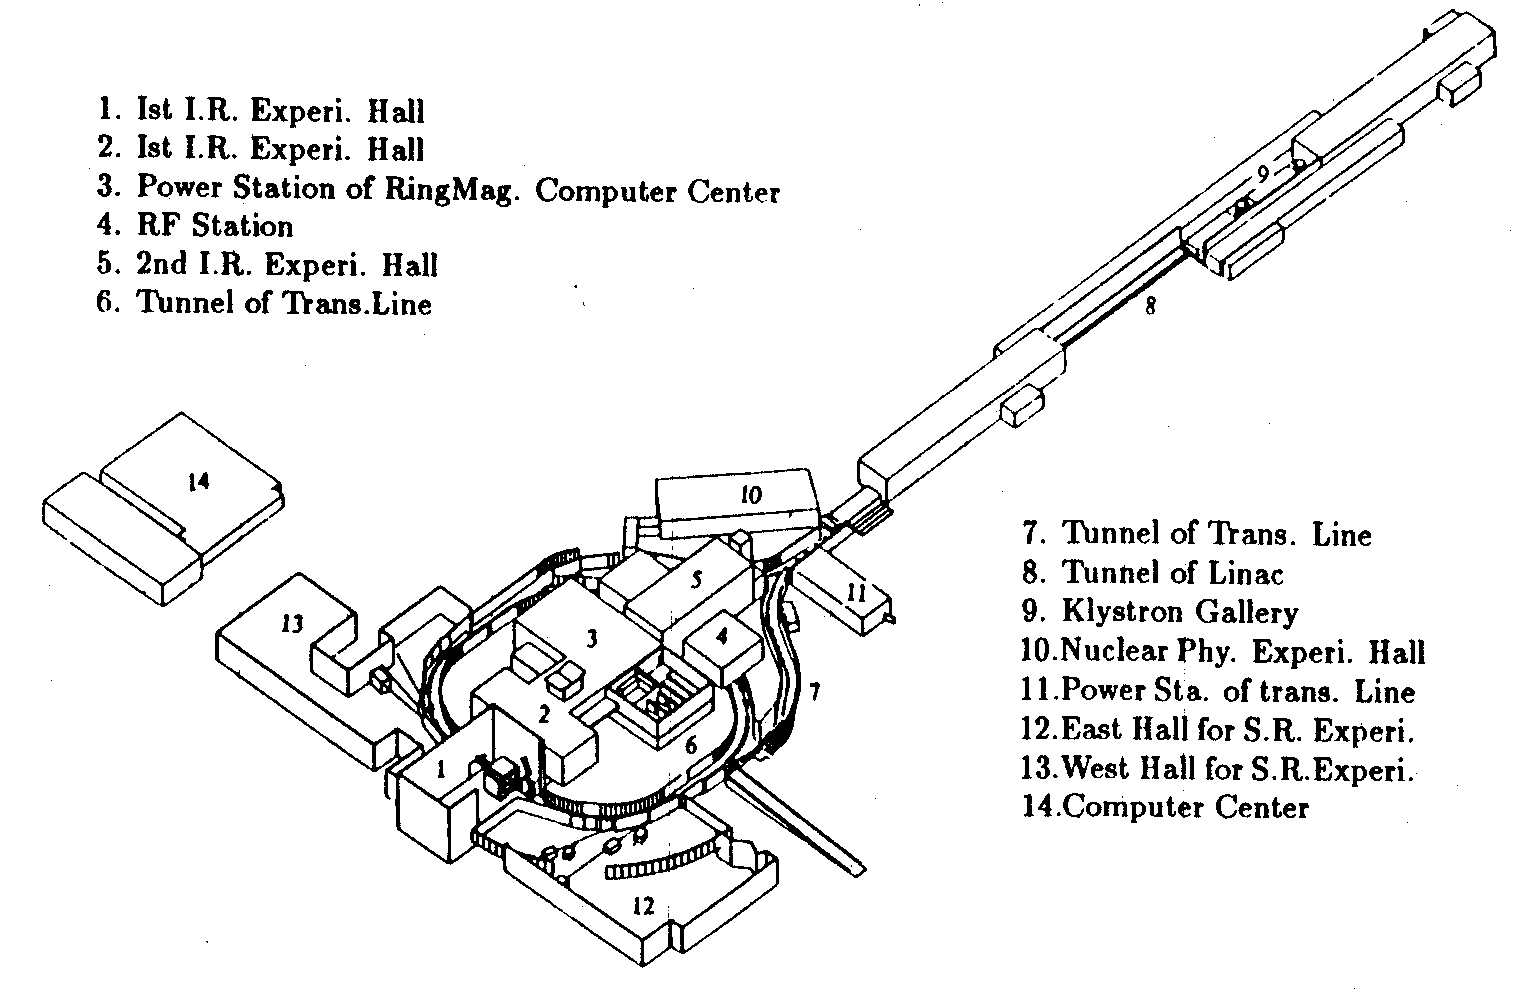
\includegraphics[width=10cm]{chap0/bepc.png}
  \caption{北京正负电子对撞机鸟瞰图}
  \label{fig:bepc}
\end{figure}

2004~年到~2008~年,BEPC~和~BESII~完成升级改造,升级后的对撞机称为~BEPCII,谱仪称为~BESIII~\cite{M.A:2010}。%升级后~BEPCII~和~BESIII~一直运行稳定。
表~\ref{tbl:BEPCII-VS-BEPC}~列出了~BEPCII~主要设计参数。
\begin{table}[htp]
  \centering
  %\footnotesize
  \caption{\label{tbl:BEPCII-VS-BEPC} BEPCII~和~BEPC~主要设计参数比较}
  \begin{tabular}{ccc}
    \hline\hline
    参数 & BEPCII & BEPC \\
    \hline
    质心能量~(GeV) & 2-4.6 & 2-5 \\
    储存环长度~(m) & 237.5 & 240.4 \\
    环的数目 & 2 & 1 \\
    高频频率~$f_{rf}$~(MHz) & 499.8 & 199.5 \\
    $2\times1.89$~GeV~(cm$^{-2}$s$^{-1}$)~下的峰值亮度 & $\sim10^{33}$ & $\sim10^{31}$ \\
    束团个数 & 2 & 1 \\
    束团流强~(A) & $2 \times 0.91$ & $2 \times 0.035$ \\
    束团间隔~(m/ns) & 2.4/8 & - \\
    束团长度~($\sigma_z$)~cm & 1.5 & $\sim 5$ \\
    束团宽度~($\sigma_x$)~$\mathrm{\mu m}$ & $\sim380$ & $\sim840$ \\
    束团高度~($\sigma_y$)~$\mathrm{\mu m}$ & $\sim5.7$ & $\sim37$ \\
    相对能散 & $5 \times 10^{-4}$ & $5 \times 10^{-4}$ \\
    对撞点束流夹角~(mrad) & $\pm 11$ & 0 \\
    \hline\hline
  \end{tabular}
  \label{tab:bepciiParam}
\end{table}

\begin{comment}
升级后的~BEPCII~是一个多束团的双环对撞机。双环指的是正负电子束流分别注入在两个彼此独立的储存环中,经加速后在对撞点发生对撞。多束团对撞可以大幅度的提高亮度。~BEPCII~的峰值亮度设计为在~1.89Gev~处达~1$\times$$10^{33}$$cm^{-2}$$s^{-1}$~。高亮度意味着可以获得大量的物理事例,为诸多基于巨大统计量的物理过程的研究和分析提供良好的实验基础。表~\ref{tbl:event-Number}~列出了~BEPCII~运行一年可以累积的各种物理事例数。
\begin{table}[h]
    \centering
    \caption{\label{tbl:event-Number} BEPCII运行一年可以积累的事例数}
    \footnotesize
    \begin{tabular}{llllc}
        \hline
        物理& 质心系能量& 峰值亮度& 物理截面& 每年产生事例数 \\
             &(Gev)      &($10^{33} $$cm^{-2}$$s^{-1}$)& (nb)\\
        \hline
        $J/\psi$& 3.097& 0.6& ~3400&  10$\times$$10^{9}$ \\
        $\tau$&   3.670& 1.0& ~2.4&    12$\times$$10^{6}$ \\
        $\psi'$&  3.686& 1.0& ~640&    3$\times$$10^{9}$\\
        D&        3.770& 1.0& ~6.5&    32$\times$$10^{6}$\\
        $D_{s}$&   4.040& 0.6& ~0.32&   1$\times$$10^{6}$\\
        $D_{s}$&   4.160& 0.6& ~1.0&    3$\times$$10^{6}$\\
        \hline
    \end{tabular}
\end{table}

\section{~BESIII~物理目标}
~BEPCII~运行在~$\tau$~-粲能区($\approx$~3~Gev),~BESIII~是运行在~BEPCII~上的大型通用探测器,通过收集~$\tau$~-粲能区的正负电子对撞产生的末态粒子进行~$\tau$~-粲物理研究。~BESIII~主要研究的物理目标有:轻强子谱、粲物理、~QCD~与~$\tau$~物理~\cite{wangyf2011}~\cite{chaokt:2009}。
\end{comment}

\section{北京谱仪(BESIII)的物理目标}
将运行在$\tau$-粲能区的~BEPC~升级到~BEPCII~,峰值亮度提高~100~倍,即每秒能获得的事例数提高~100~倍,同时新建一个与高亮度相对应的高精度探测器~BESIII~,无疑对该能区高能度的物理研究提供了很好的条件,将有力地促进粒子物理的进一步发展。

BEPCII~的峰值亮度设计为在~1.89~Gev~处达到~1$\times$$10^{33}$$cm^{-2}$$s^{-1}$~,为$\tau$-粲能区有史以来的最高值,预期会获得前所未有的大量物理事例,为我们得到重要物理结果提供了机会。考虑到加速器的亮度、运行时间、各类事例的产生截面、探测器的最大覆盖立体角及正负电子束流的能散度,BEPCII~运行一年可以积累的各种物理事例数~\cite{yuancz:2002}~见表~\ref{tbl:event-Number}~

\begin{table}[h]
    \centering
    \caption{\label{tbl:event-Number} BEPCII运行一年可以积累的事例数}
    \footnotesize
    \begin{tabular}{llllc}
        \hline
        物理& 质心系能量& 峰值亮度& 物理截面& 每年产生事例数 \\
             &(Gev)      &($10^{33} $$cm^{-2}$$s^{-1}$)& (nb)\\
        \hline
        $J/\psi$& 3.097& 0.6& ~3400&  10$\times$$10^{9}$ \\
        $\tau$&   3.670& 1.0& ~2.4&    12$\times$$10^{6}$ \\
        $\psi'$&  3.686& 1.0& ~640&    3$\times$$10^{9}$\\
        D&        3.770& 1.0& ~6.5&    32$\times$$10^{6}$\\
        $D_{s}$&   4.040& 0.6& ~0.32&   1$\times$$10^{6}$\\
        $D_{s}$&   4.160& 0.6& ~1.0&    3$\times$$10^{6}$\\
        \hline
    \end{tabular}
\end{table}

根据以上估计的~BESIII~能够获取的事例数及~BESIII~探测器的性能指标,我们组织了国内外几十位理论与实验物理学家全面回顾了轻强子谱、粲偶素物理、粲物理、QCD与$\tau$物理等方面研究的现状,提出了~BESIII~的物理研究目标,完成了黄皮书~Physics at BESIII。~\cite{chaokt:2009}~\cite{wangyf2011}~

\section{~BESIII~探测器}
谱仪是各种粒子探测器的组合,通过观察和测量粒子对撞后产生的次级粒子的动量、能量、位置、质量等各种参数,重建各类反应过程,进而研究物理的基本性质。~BEPCII~是高亮度、多束团的对撞机,其设计亮度比~BEPC~高~100~倍,高亮度带来的高统计量使~BESIII~的统计误差减少到~BESII~的~1/10~,这些都需要有一个与之相匹配的高质量的探测器。因此~BESIII~探测器需要满足多束团、高计数率下的取数要求;~BESIII~探测器的系统误差应该减少到之前~BESII~的~1/10~下才匹配。基于此,~BESIII~的设计必须满足以下要求:
\begin{itemize}
\item{10MeV~到~2.5Gev~内,有好的能量分辨率,位置分辨率和光子识别能力;}
\item{50Mev~到~2.5Gev~内,能精确的测量带电粒子的动量和方向;}
\item{50Mev~到~2.5Gev~内,有好的粒子鉴别能力;}
\item{电子学和数据获取系统能够适应多束团模式和高数据率取数。}
\end{itemize}

为满足以上要求,~BESIII~探测器的最终设计为:
\begin{itemize}
\item{采用单丝分辨率好于~130$\mu$m~的小单元氦基气体漂移室作为径迹探测器;}
\item{采用~$C_{s}$I~晶体量能器探测鉴别光子和电子;}
\item{采用塑料闪烁体构成的飞行时间探测器作为粒子鉴别探测器;}
\item{采用场强为~1.0T~的超导螺线管磁铁;}
\item{采用阻性板探测器的~$\mu$~子室;}
\item{采用基于流水线技术的前端电子学系统适应多束团模式和高数据率的数据获取系统。}
\end{itemize}

表~\ref{tbl:BESIII-VS-BESII}~列出了~BESIII~各组成部分的主要性能。
\begin{table}[h]
	\centering
	\caption{\label{tbl:BESIII-VS-BESII} BESIII~和~BESII~探测器的比较}
    \scalebox{0.8}{
	%\footnotesize
	\begin{tabular}[c]{lll}
		\hline
		子系统& ~BESIII~& ~BESII~ \\
		\hline
        \multirow{3}{4cm}{主漂移室}&   $\sigma_{xy}$~ = ~130~ $\mu$m & 250~$\mu$m \\
                &   $\Delta$p/p = 0.5~$\%@$1~Gev&  2.4~$\%$@1~Gev \\
                &  $\sigma_{dE/dx}$ = 6~$\%$&      8.5~$\%$       \\
        \hline
        \multirow{2}{4cm}{电磁量能器}&   $\sigma_{E}$/E = 2.5~$\%@$1~Gev&  20~$\%$@1~Gev \\
                  &   $\sigma_{x,y}$ = 0.6~cm@1~Gev&   3~cm@1~Gev \\
        \hline
        \multirow{2}{4cm}{飞行时间探测器}&  $\sigma_{T}$=100~ps(桶部)& 180~ps(桶部)\\
                     &  $\sigma_{T}$=110~ps(端盖)& 350~ps(端盖)\\          
        \hline
        $\mu$子计数器&  9~层& 3~层  \\
        \hline
        磁铁& 1.0T~& 0.4~T\\
		\hline
	\end{tabular}
    }
\end{table}

%图~\ref{fig:BESIII}~给出了BESIII总体结构端面视图。
\begin{figure}[!h]
  \centering
  \includegraphics[width=10cm,angle=90]{chap0/bes_view.eps}
  \caption{~BESIII~总体结构端面视图}
  \label{fig:BESIII}
\end{figure}
图~\ref{fig:BESIII}~给出了北京谱仪总体结构端面视图。
由内到外分别是:束流管~(Beam Pipe)~,主漂移室~(Main Drift Chamber,MDC)~,飞行时间探测器~(Time of Flight Counter,TOF)~,电磁量能器~(Electromagnetic Calorimeter,EMC)~,超导磁铁~(Superconducting Magnet,SM)~,~$\mu$~子探测器。
此外,~BESIII~还具有用于监视谱仪各部分的运行并记录其运行参数的分布式的慢控制系统~(slow control system)~;高保真读出各探测器信号的电子学系统~(read-out electronics system)~;在线选择感兴趣的事例的触发系统~(trigger system)~;在线数据获取系统~(data acquisition system,DAQ)~,以及用于处理记录下来的数据的离线数据系统~(offline data processing system)~。
%\subsection{主漂移室(Main Drift Chamber)}
\subsection{主漂移室}
主漂移室是~BESIII~的主要子探测器之一:主要任务是:

\begin{itemize}
\item{精确测量从相互作用点产生的带电粒子动量和方向;}
\item{为带电粒子的粒子鉴别提供足够好的电离能损~(dE/dx)~测量;}
\item{对带电粒子的测量有尽量大的立体角覆盖~(~97$\%$ 4$\pi$)~}
\item{对低动量带电粒子径迹有尽可能大的重建效率;}
\item{为带电粒子的一级硬件触发提供信号。}
\end{itemize}

%主漂移室的主要任务:为$\tau$-charm能区产生的带电粒子提供优秀的动量测量能力,同时提供好的电离能损的测量能力;
%提供一级触发的信号,用来筛选好的物理事例,压缩本底。

主漂移室中带电粒子的动量测量依赖于其在漂移室磁场中飞行轨迹的测量,具体就是带电粒子在漂移室中击中位置越多,重建处的粒子的飞行径迹就越确定,测得的动量就越准确。对于低动量带电粒子,影响动量测量精度的是在飞行过程中与探测器中的物质发生的多次库仑散射。为减少多次库仑散射的影响,需要尽可能的选用低原子序列的材料作为漂移室的气体和场丝。

漂移室采用小单元结构,使用镀金铝丝作为场丝,使用~$H_{e}$/$C_{3}H_{8}$(60/40)~作为工作气体。立体角覆盖~$\Delta\Omega/4\pi$=0.93~,单丝的位置精确度为~130$\mu$m~.对于动量为~1~Gev~的带电粒子动量分辨率为~0.5~$\%$左右;在粒子的入射角为~$90\degree$~,~dE/dx~分辨~6~$\%$下,~$\pi/K$~的分辨能力(3$\sigma$)可达到~770~Mev/c。
\begin{figure}[!h]
  \centering
  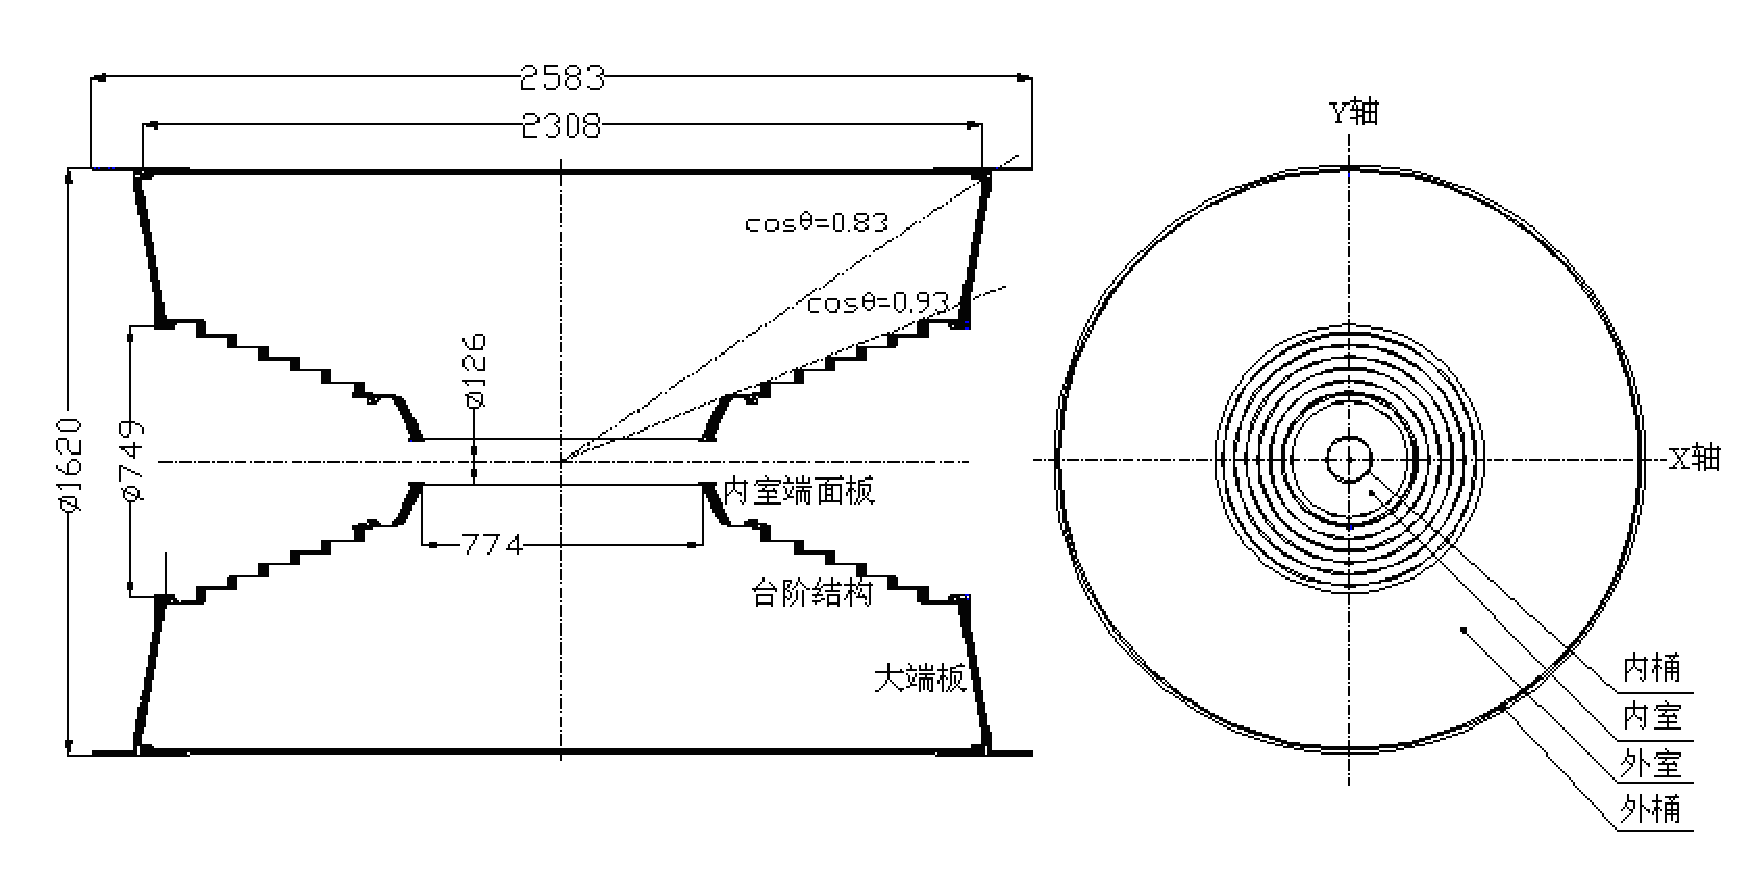
\includegraphics[width=10cm]{chap0/mdc-global.eps}
  \caption{主漂移室的结构示意图}
  \label{fig:mdc-global}
\end{figure}
%图~\ref{fig:mdc-global}~给出了MDC的结构示意图。

%\subsection{飞行时间探测器(Time of Flight Counter)}
\subsection{飞行时间探测器}
BESIII的飞行时间探测器主要是用来做粒子鉴别。鉴别能力大小由相同动量粒子的飞行时间差和自身的时间分辨率所决定。
飞行时间探测器由桶部和端盖构成。其中,桶部部分固定在主漂移室上,采用双层结构,每层~88~块,每块长~2.32~m,厚~5~cm,截面为梯形。信号由双端读出。端盖固定在端盖电磁量能器上,有东西两部分,每部分~48~个扇形闪烁体。桶部的立体角覆盖为~$|$cos($\theta$)$|<$0.83~;端盖的立体角覆盖为~0.85$<|$cos($\theta$)$|<$0.95~;桶部的设计时间分辨是~100~ps,在粒子的入射角为~$90\degree$~,~$\pi/K$~的分辨能力~(3$\sigma$)~大约达到~700~Mev/c。

%\subsection{电磁量能器(Electromagnetic Calorimeter)}
\subsection{电磁量能器}

电磁量能器用来精确测量的光子的能量和提供触发中性事例的信号。在动量大于~200~Mev/c下有好的~e/$\pi$~的分辨能力。EMC~有桶部和端盖组成,有~6240~块晶体,桶部内半径~94~cm,内长~275~cm,覆盖角~$|$cos($\theta$)$|<$0.82~;端盖覆盖角为~0.83$<|$cos($\theta$)$|<$0.93~。EMC的能量覆盖范围为~20~Mev~~2~Gev,在~1~Gev下,能量分辨率为~$\Delta$E/$\sqrt E$=2.5$\%$~,位置分辨率为~$\sigma$=0.6cm/$\sqrt E$(E in Gev)~。
\begin{figure}[!h]
  \centering
  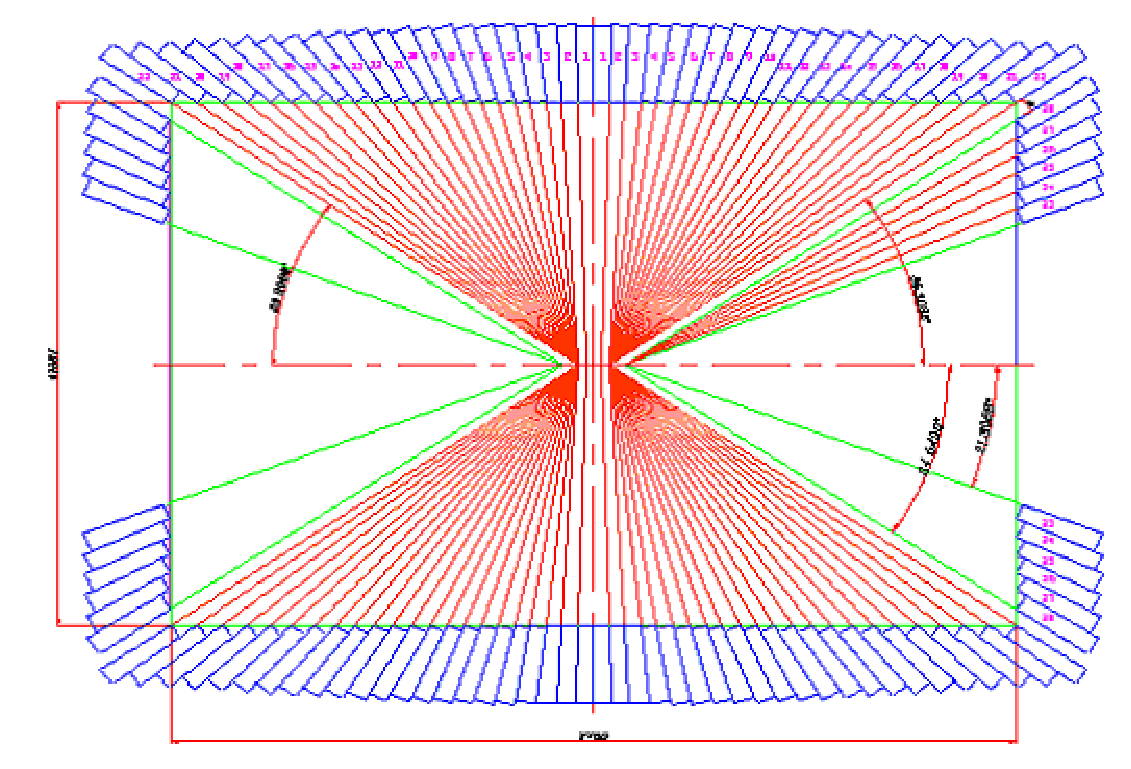
\includegraphics[width=10cm]{chap0/besiii-emc.eps}
  \caption{EMC晶体分布示意图}
  \label{fig:besiii-emc}
\end{figure}
%图~\ref{fig:besiii-emc}~给出了MDC的结构示意图。

\subsection{$\mu$子探测器}

~$\mu$~子探测器位于BESIII探测器的最外层,包括~$\mu$~子探测器和强子吸收体主要功能是从末态的带电粒子中区分出~$\mu$~子和$\pi$等其他带电强子。~$\mu$~子探测器选用的是阻性板计数器(resistive plate counters,RPC)。~$\mu$~子探测器设计成桶部和端盖两部分以增大立体角覆盖。桶部~$\mu$~子探测器内半径为~170~cm,外半径为~262~cm,共有8层厚度为~3-8~cm的RPC和吸收铁,按照八角形排列。吸收铁和~RPC~采用夹层结构,两层铁之间夹缝为~4~cm,~RPC~位于其中。端盖采用~8~层吸收铁和~8~层RPC的夹层结构。桶部端盖总的覆盖立体角为~0.85~,其中桶部最内层为~0.75~,最外层为~0.60~。动量大于~0.4~Gev的~$\mu$~子在不同入射角度的探测效率均可达到~95$\%$~。

%\subsection{超导磁铁(Superconducting Magnet)}
\subsection{超导磁铁}

超导磁铁是~BESIII~的一个重要组成部分,利用轭铁作为磁场回路提供高强度和一定均匀度的轴向磁场,用来供~MDC~测量带点粒子的径迹。磁铁长~4.91~m,内直径~2.75~m,为直径为~3.4~m,线圈长度~3.52~m,中心直径~2.95~m。轭铁分为桶部和端盖两部分,除了作为磁场回路外,也做~$\mu$~子探测器的吸收体。较高的磁场强度可以提高~MDC~中带电粒子的动量分辨率,但过高的磁场长度会对低动量的径迹测量带来困难。综合考虑,超导磁铁的中心磁场强度设计为~(0.0,0.0,1.0)~T,径迹区内磁场的不均匀读~$\leq5\%$~,磁场测量的精度~$\leq0.1\%$~。

\section{飞行时间探测器}

飞行时间探测器是用来测量带电粒子的飞行时间。具体来说,测量的时间是粒子到达飞行时间探测器的时刻。和束流在对撞顶点发生对撞的时刻(~$t_{0}$~)之间的时间间隔,就是粒子从对撞点飞行到飞行时间探测器的时间。(见图~\ref{fig:TOF-theory}~,图~\ref{fig:traw}~)
%粒子鉴别正是利用得到的测量飞行时间结合利用主漂移室测量的粒子动量~p~和飞行径迹~$\L$~得到的预期飞行时间完成的。

%图~\ref{fig:TOF-theory}~给出了TOF探测器原理示意图。
\begin{figure}[!h]
  \centering
  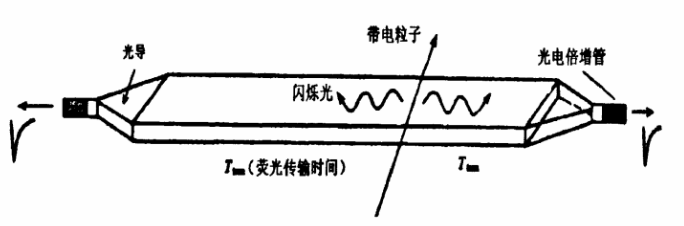
\includegraphics[width=0.9\textwidth]{chap0/TOF-theory.png}
  \caption{TOF探测器原理示意图}
  \label{fig:TOF-theory}
\end{figure}

\begin{figure}[!h]
  \centering
  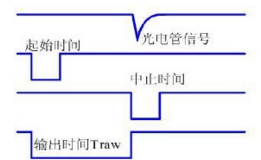
\includegraphics[width=0.5\textwidth]{chap0/traw.png}
  \caption{TOF探测器测量的飞行时间}
  \label{fig:traw}
\end{figure}

带电粒子从对撞顶点到击中~TOF~的预期飞行时间~$t_{exp}$~由公式~\ref{eq:0.1}~给出,其中~$L$~是带电粒子从对撞顶点到击中~TOF~的飞行距离。$\beta$~是带电粒子的飞行速度,由公式~\ref{eq:0.1}~给出,其中~m~是带电粒子的质量,~p~是带电粒子的动量。L~和~p~都是由主漂移室测量得到的。

\begin{align}
t_{exp}=L/\beta c 
\label{eq:0.1}\\
\beta=p/\sqrt {p^{2}+m^{2}}
\label{eq:0.2}
\end{align}

%由公式~\ref{eq:0.1}~和~\ref{eq:0.2}~即可求出粒子的质量$m_{0}$,鉴别出带电粒子。

对于动量都等于p,质量分别为$m_{1}$和$m_{2}$的两个带电粒子,它们的飞行时间差的具体由公式~\ref{eq:0.4}~给出。
\begin{align}
\frac{1}{\beta^{2}_{2}}-\frac{1}{\beta^{2}_{1}}=\frac{m^{2}_{2}-m^{2}_{1}}{p^{2}}
\label{eq:0.3}\\
t_{2}-t_{1}=\frac{L}{c\beta_{2}}-\frac{L}{c\beta_{1}}=(\frac{L}{c})(\frac{m^{2}_{2}-m^{2}_{1}}{p^{2}})(\frac{\beta_{1}\beta_{2}}{\beta_{1}+\beta_{2}})\leq(\frac{L}{c})(\frac{m^{2}_{2}-m^{2}_{1}}{2p^{2}})
\label{eq:0.4}
\end{align}
由公式~\ref{eq:0.4}~可知,粒子飞行距离越长,粒子动量越小,则粒子的鉴别能力越好。

\subsection{粒子鉴别}
飞行时间探测器主要物理目标是粒子鉴别(particle identification),其能力大小主要由相同动量粒子的飞行时间差和飞行时间探测器的时间分辨所决定。它通过测量带电粒子在主漂移室内的飞行时间,结合主漂移室测得粒子的动量和径迹,根据不同粒子的质量不同,从而辨别粒子的种类;同时它也参与第一级触发判选,而且可以利用不同探测器输出信号之间的时间关系来排除宇宙线本底。飞行时间探测器的飞行时间差随内半径的变大而增加;时间分辨分别由正负电子对撞的起始时间推算精度和粒子打到飞行时间探测器后测量的截止时间的精度决定,其中飞行时间探测器的本征时间分辨率是主要因素。

影响TOF的时间分辨的因素很多,总的时间分辨$\sigma$可以写成:
\begin{displaymath}
\sigma=\sqrt{\sigma_{TOF}^{2}+\sigma_{bunch-time}^{2}+\sigma_{bunch-length}^{2}+\sigma_{Z-position}^{2}+\sigma_{electronics}^{2}+\sigma_{expect}^{2}+\sigma_{time-walk}^{2}}
\end{displaymath}

其中$\sigma_{TOF}$是TOF的本征时间分辨率,反映了探测器的主要性能;$\sigma_{bunch-time}$表示束团时间不确定性;$\sigma_{bunch-length}$表示束团长度形成的对撞时刻的不确定性;$\sigma_{Z-position}$来源于粒子击中闪烁体的Z向定位的不确定性,会导致光在闪烁体内的传输时间不确定;$\sigma_{electronics}$表示来自电子学时间测量的不确定性;$\sigma_{expect}$表示来自预期飞行时间的不确定性;$\sigma_{time-walk}$表示来源于电子学阈效应的时间修正过程。

表~\ref{tbl:TOF-expect-sigma}~列出了预期的TOF时间分辨率分析。
\begin{table}[h]
    \centering
    \caption{\label{tbl:TOF-expect-sigma} 预期的TOF时间分辨率分析}
    \footnotesize
    \begin{tabular}{lll}
        \hline
        时间分辨项目& 桶部时间分辨率& 端盖时间分辨率 \\
        \hline
        单层TOF本征时间分辨率(对1Gev的$\mu$子)& 80-90ps&        80ps \\
        束团时间的不确定性&                     5ps&            5ps \\
        束团长度的不确定性&                     15mm,35ps&      15mm,35ps\\
        MDC外推的定位精度&                      5mm,33ps&       5-10mm,47-95ps\\
        电子学测量的精度&                       25ps&           25ps\\
        预期飞行时间精度&                       30ps&           40ps\\
        时幅修正&                               10ps&          10ps  \\
		单层TOF总的时间分辨率&                   100-110ps&     110-137ps           \\
		双侧TOF总的时间分辨率&                   80-90ps&       无                \\       
        \hline
    \end{tabular}
\end{table}

\subsection{桶部TOF和端盖TOF}
桶部TOF的径向半径从~810~mm到~925~mm。桶部闪烁体选用的是长度为~2.3~m,宽度约为两英寸,厚度为~5~cm,型号为~BC408~闪烁体。
%图~\ref{fig:TOF}~给出了~TOF~的结构示意图。
\begin{figure}[!h]
  \centering
  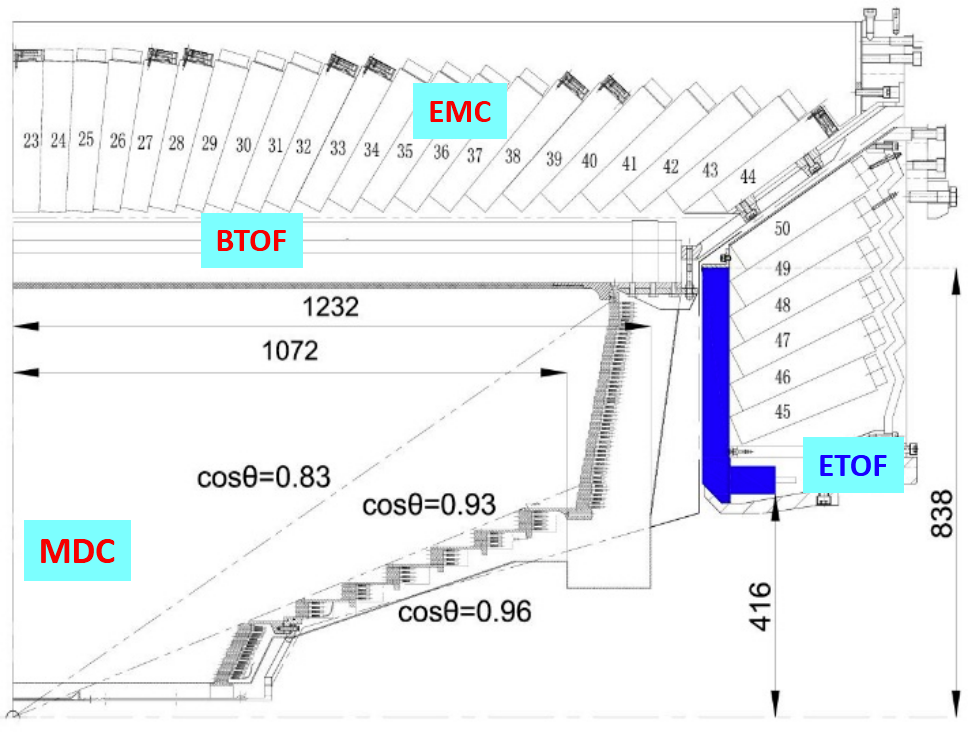
\includegraphics[width=0.8\textwidth]{chap0/TOF.png}
  \caption{飞行时间探测器结构 BTOF指的桶部TOF,ETOF指的端盖TOF}
  \label{fig:TOF}
\end{figure}

端盖TOF的塑料闪烁体的长度短于桶部~TOF~,选用的是~BC404~信号的闪烁体,可以充分发挥~BC404~光产额高,时间快的优势。
\begin{figure}[!h]
  \centering
  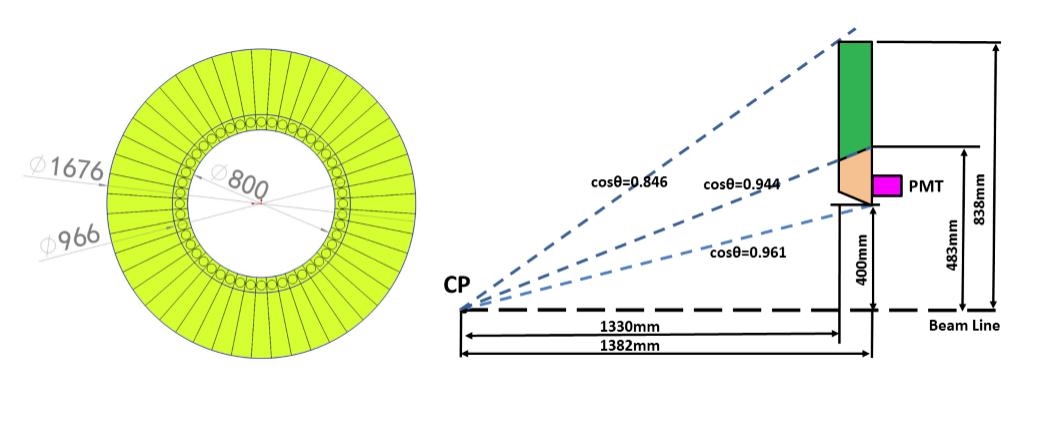
\includegraphics[width=0.9\textwidth]{chap0/ETOF.png}
  \caption{端盖TOF几何尺寸与空间安排}
  \label{fig:ETOF}
\end{figure}
%图~\ref{fig:ETOF}~给出了ETOF的结构示意图。
\subsection{TOF的电子学系统}
飞行时间探测器的电子学系统的基本功能是进行带电粒子的飞行时间测量。简单讲,测量的是正负电子对撞时刻与次级带电粒子击中飞行时间探测器刻度之间的时间间隔。现代粒子物理实验测量时间最有效的定时方法依然是快前沿定时。为了校正前沿定时方法中时间游走(time-walk)效应带来的测量误差,系统还必须对光电倍增管输出信号的幅度(电荷)进行测量。此外,飞行时间探测器的另一个主要功能是提供粒子击中的快时间响应信号给触发系统。
基于此,~TOF~电子学系统需要完成三项基本功能:时间测量,电荷测量,提供粒子击中的快时间响应。

TOF的读出电子学系统由前置放大器部分和读出电子学VME系统组成。前置放大器对光电倍增管输出的探测器信号进行~10~倍的放大,输出的差分信号经过~18~米的差分屏蔽电缆送入到读出电子学VME系统进行数字化处理。

TOF前端电子学系统采用的是~VME$\quad$9U~作为~TOF~前端读出电子学系统的硬件平台;采用全差分的信号处理和传输技术;对时间和电荷量的测量采用统一的数字化处理。时间测量采用的是快前沿定时甄别+~HPTDC~数字化技术。~TOF~采用阈值甄别技术,只有高于阈值的信号才能被电路输出。~HPTDC~时间测量直接测量的是粒子到达探测器的“hit”时间。飞行时间需要通过离线数据分析,得到对撞时间所对应的的时钟的时刻,再通过束团之间固定的时间关系,然后相减得到。

\section{论文选题的意义}

通过触发判选和在线选择的事例,由在线数据系统获取系统以二进制文件的形式记录下来。这种数据称为原始数据,主要包含的是探测器的电子学信号的时间和幅度信息。这样的原始数据是不能直接被物理分析使用的。原始数据需要经过一定的处理才能得到物理分析所需要的包括能量,动量,运动方向等信息。经过的这些处理就是离线刻度和重建。离线刻度可以消除实验中的各种外部条件和探测器自身条件对电子学信号和物理测量量之间转化带来的影响。离线刻度对每个不同的子探测器分别进行,生成刻度常数。重建就是利用刻度常数将原始的数据转化为粒子的动量,能量,运动方法等物理量,生成重建数据。物理分析就是利用重建数据进行的。~\cite{wangyf2011ww}

BESIII实验在2015年夏季完成端盖飞行时间探测器的升级改造,用多气隙电阻性板室(Multi-gap Resistive Plate Chamber,简称MRPC)替代现有的闪烁体。MRPC探测器具有较小的时间分辨,同时又能保证足够的探测效率。为与探测器硬件升级相适应的离线数据处理和分析系统需要完成~MRPC~端盖~TOF~的软件开发和数据处理方面的研究。

对端盖~MRPC-TOF~探测器的刻度方法进行研究,建立一套稳定并行之有效的刻度流程,满足数据刻度和重建的需要,把优秀的探测器指标转化为物理分析中的优良的粒子鉴别能力,是论文研究的主要内容。
研究采用了样条插值和构造公式两种方法。下面的章节会详细探讨在研究中遇到的难点,以及采用何种方法进行解决。

\section{MRPC刻度方法国内外现状}

美国布鲁克海文国家实验室~(BNL)~的相对论重离子对撞机~RHIC~上的螺旋径迹探测器STAR实验~\cite{ruanlj:2005}~\cite{wuj:2005}~\cite{wangy:2010}的主要科学目标是寻找可能存在的新物质形态夸克-胶子等离子体,并研究极端高温、高密下的强相互作用物质的演化动力学。欧洲核子中心(CERN)的大型强子对撞机LHC上的大型离子对撞机~ALICE~实验~\cite{A.Alici:2012}~\cite{A.Alici:2014}是在极端能量密度下研究强相互作用物理,寻找夸克胶子等离子体,研究量子色动力学。这两个实验都采用MRPC做为飞行时间探测器。

\begin{comment}
~STAR~的~TOF~由~3840~块~MRPC~组成,每块有~6~个读数条。刻度样本选择的是动量在~0.3—0.6Gev/c~的~$\pi$~介子。由于信号在读出条内的反射,每个电子学读出通道的~TOT~(time-over-threshold~\cite{Shao:2009aa},简称TOT)分布存在多峰,且各不相同,时幅修正的刻度采用样条拟合(spline-fit)的方法。信号在读出条上的传输时间依赖信号传播距离,击中位置的修正只考虑沿读出条方向的效应。扣除起始时间晃动~55~ps后,时间分辨为~75~ps~\cite{Shao:2009aa}。

~ALICE~的~TOF~由~1593~块~MRPC~组成,每块面积为~7.4~cm$\times$~120~cm,每个模块~96~个读出端,每个读出端面积为~2.5~cm$\times$~3.5~cm。刻度样本需要完整的径迹重建。~TOF~刻度分为三个步骤:(1)一个整体的偏移;(2)每个电子学通道的偏移;(3)每个电子学通道的时幅修正。时幅修正采用的是~TOT~的~5~阶多项式拟合。扣除事例起始时间的影响后,时间分辨为~80~ps~\cite{A.A:2005}。
\end{comment}

\subsection{STAR实验的MRPC飞行时间探测器离线数据的刻度方法}
\begin{figure}[!h]
  \centering
  \includegraphics[width=0.9\textwidth]{chap0/STAR-MRPC.png}
  \caption{STAR实验的MRPC模块结构图。(a)长边视图;(b)短边视图}
  \label{fig:STAR-MRPC}
\end{figure}

STAR实验的圆柱型~TOF~覆盖面积大约有64$m^{2}$,整个系统由120个托盘,每个托盘有32个MRPC模块组成,每个MRPC模块有6个读数条。每个读数条长6.0cm,宽3.1cm~\cite{wangy:2010}。图~\ref{fig:STAR-MRPC}~给出了STAR实验的MRPC模块的结构图。实验采用基于CERN开发的NINO芯片的前端电子学系统,高性能的时间-数字转化电路(high-performance time to digital convertor,HPTDC)可以同时测量信号过阈的前沿和后沿的时间。其中前沿用于定时,后沿和前沿之间的间隔为过阈时间(TOT),用于对前沿时间的晃动进行校准。

STAR关于MRPC-TOF的刻度方法分为5步:
\begin{itemize}
\item{挑选样本:选择动量在0.3-0.6Gev $c^{-1}$,dE/dx$\textless2.5KeV cm^{-1}$的$\pi$(纯度$\geq99$$\%$)}
\item{对事例起始时间时间进行修正,按每个读出通道进行修正}
\item{对过阈时间进行修正,按每个读出通道进行修正}
\item{对击中读数条的位置进行修正,因为每个读数条信号的传播速度并不一致,按每个读出通道进行修正。(这里只考虑沿着读数条传播方向的效应)}
\item{对第三步和第四步进行第二次修正,来提高修正效应}
\end{itemize}

具体每步修正采用的是样条插值(spline fit)的方法。
图~\ref{fig:STAR-TOT}~是STAR实验测得的不同模式的过阈时间的分布。左边的图和中间的图可以看出很明显的多峰现象。
\begin{figure}[!h]
  \centering
  \includegraphics[width=0.9\textwidth]{chap0/STAR-TOT.png}
  \caption{STAR实验测得的不同模式的过阈时间的分布。前两幅图可以明显看出多峰现象}
  \label{fig:STAR-TOT}
\end{figure}

图~\ref{fig:STAR-time}~是STAR实验测得的不同过阈时间模式下的原始时间的分布。
\begin{figure}[!h]
  \centering
  \includegraphics[width=0.9\textwidth]{chap0/STAR-time.png}
  \caption{HPTDC测量的原始时间的分布。对应不同的过阈时间模式}
  \label{fig:STAR-time}
\end{figure}

图~\ref{fig:STAR-fit-TOT}~是STAR实验对过阈时间修正的方法,对于不同的过阈时间模式采用的都是样条插值的方法。
\begin{figure}[!h]
  \centering
  \includegraphics[width=0.9\textwidth]{chap0/STAR-fit-TOT.png}
  \caption{对应不同模式的过阈时间的样条插值}
  \label{fig:STAR-fit-TOT}
\end{figure}

图~\ref{fig:STAR-fit-t0}~表示插值拟合对事例起始时间的修正(这个修正是放在修正过阈时间和击中位置之前的)。图~\ref{fig:STAR-fit-z}~表示插值拟合对击中位置的修正。
\begin{figure}[!h]
\begin{minipage}[!h]{0.5\linewidth}
\centering
\includegraphics[width=0.9\textwidth]{chap0/STAR-fit-t0.png}
\subcaption{插值方法拟合起始时间}
\label{fig:STAR-fit-t0}
\end{minipage}
\hfill
\begin{minipage}[!h]{0.5\linewidth}
\centering
\includegraphics[width=0.9\textwidth]{chap0/STAR-fit-z.png}
\subcaption{插值方法拟合击中位置}
\label{fig:STAR-fit-z}
\end{minipage}%
\caption{插值方法拟合事例起始时间和击中位置}
\end{figure}

图~\ref{fig:STAR-res}~是STAR实验修正后得到的时间分辨(过阈时间和击中位置都是修正了两次),约89ps,扣除起始时间的晃动(~55ps),最终的MRPC的时间分辨是75ps。
\begin{figure}[!h]
  \centering
  \includegraphics[width=0.9\textwidth]{chap0/STAR-res.png}
  \caption{最终修正后得到的时间分辨 (a)总的时间分辨;(b)每个道的时间分辨}
  \label{fig:STAR-res}
\end{figure}

\subsection{ALICE实验的MRPC飞行时间探测器离线数据的刻度方法}
~ALICE~的~TOF~由~1593~块~MRPC~组成,每块面积为~7.4~cm$\times$~120~cm,每个模块~96~个读出端,每个读出端面积为~2.5~cm$\times$~3.5~cm。刻度样本需要完整的径迹重建。~TOF~刻度分为三个步骤:(1)一个整体的偏移;(2)每个电子学通道的偏移;(3)每个电子学通道的时幅修正。

图~\ref{fig:ALICE-offset}~对应上面的前两步。左图表示的是一个整体的偏移情况,右图表示的是拟合获取单个电子学通道偏移值。
\begin{figure}[!h]
  \centering
  \includegraphics[width=0.9\textwidth]{chap0/ALICE-offset.png}
  \caption{左图:LHC实验在2012年整体的电子学通道的时间偏移情况;右图:一个电子学通道的时间偏移的拟合}
  \label{fig:ALICE-offset}
\end{figure}

图~\ref{fig:ALICE-fit-TOT}~对应第三步的修正。其中对于时幅修正采用的是多项式拟合。
\begin{figure}[!h]
  \centering
  \includegraphics[width=0.9\textwidth]{chap0/ALICE-fit-TOT.png}
  \caption{时幅修正。径迹选择的是0.5$<$p$<$1.5Gev。上方:空的直方图和阴影的直方图分别表示拟合后和之后前的情况;下方:4个对数条拟合时幅修正的情况,采用的是多项式拟合}
  \label{fig:ALICE-fit-TOT}
\end{figure}

图~\ref{fig:ALICE-res}~对应第三步的修正。选择的是动量在0.95$<$p$<$1.05Gev/c范围内的$\pi$介子作为刻度样本。扣除起始时间的晃动后时间分辨是80ps。
\begin{figure}[!h]
  \centering
  \includegraphics[width=0.9\textwidth]{chap0/ALICE-res.png}
  \caption{ALICE实验的MRPC的时间分辨;选择的是动量在0.95$<$p$<$1.05Gev/c范围内的$\pi$介子作为刻度样本}
  \label{fig:ALICE-res}
\end{figure}

\section{论文的结构}
根据论文的主要内容,论文的结构安排如下:
第一章是论文的前言部分,简单介绍了粒子物理学和~BESIII~实验的基本知识,然后介绍了论文选题的背景和意义,以及国内外关于MRPC探测器数据刻度方法。
第二章介绍了~BESIII~实验的~MRPC~端盖~TOF~,刻度重建流程,以及刻度中的重点和难点问题。
第三章介绍利用插值方法对~BESIII~的~MRPC~端盖~TOF~进行离线数据刻度的研究。
第四章介绍利用构造公式对~BESIII~的~MRPC~端盖~TOF~进行离线数据刻度的研究。
第五章介绍利用双端数据采用插值和构造公式两种方法对~BESIII~的~MRPC~端盖~TOF~进行离线数据刻度的研究。
第六章介绍了刻度公式的适用性问题,以及过阈时间和击中位置关联项的问题。
第七章对论文的内容进行总结。












  % !TeX root = ../main.tex
% !TEX root = ../main.tex
% -*- root: ../main.tex -*-
% -*- program: pdflatex -*-
\chapter{~MRPC~端盖~TOF~离线数据}
原来的端盖~TOF~采用的塑料闪烁体,分东西两部分,每部分单层结构,闪烁体为扇形,光电倍增管垂直耦合,放置于扇形闪烁体的内端。每部分有~48~块。
图~\ref{fig:end-TOF-sigma}~给出了~端盖TOF~的时间分辨。
其中对于~Bhabha~事例样本,时间分辨为~148~ps;对于双~$\mu$~子事例,时间分辨为~110~ps,\cite{zhaoc:2011}。分辨率的不同主要来自不同粒子与探测器材料不同作用的差别,由于~$\mu$~子散射小,击中塑料闪烁体的位置不确定性较小,相比较~Bhabha~事例而言(位置的不确定性以及多次散射效应)非本征的时间分辨贡献较小,因而时间分辨相对较好。
\begin{figure}[!h]
  \centering
  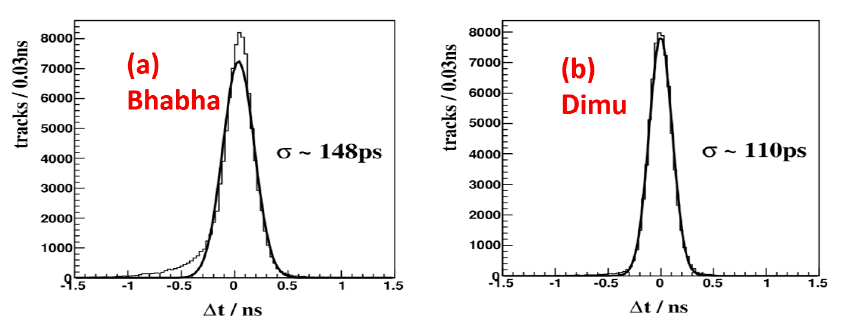
\includegraphics[width=0.9\textwidth]{chap1/end-TOF-sigma.png}
  \caption{端盖~TOF~的时间分辨:(a)电子和(b)~$\mu$~子}
  \label{fig:end-TOF-sigma}
\end{figure}
图~\ref{fig:end-TOF-eff}~给出了端盖~TOF~的各探测单元的效率。探测效率大致为~96$\%$~\cite{wangxz2016}。
\begin{figure}[!h]
  \centering
  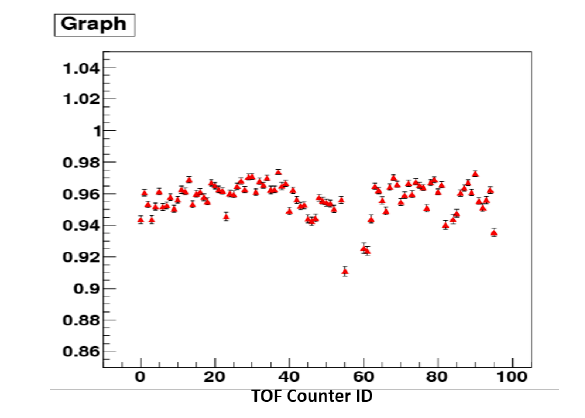
\includegraphics[width=0.8\textwidth]{chap1/end-TOF-eff.png}
  \caption{端盖~TOF~的各探测器单元的效率}
  \label{fig:end-TOF-eff}
\end{figure}

对于端盖~TOF~而言,由于多次散射,导致性能相比较桶部而言,明显较差。~端盖TOF~的~$\pi/K$~的分辨能力如图~\ref{fig:end-TOF-PID}~\cite{zhaoc:2011}所示,在~95.4$\%$(2$\sigma$)~正确率下,$\pi/K$~介子的鉴别能力基本可以达到~1.1~GeV以内。

\begin{figure}[!h]
  \centering
  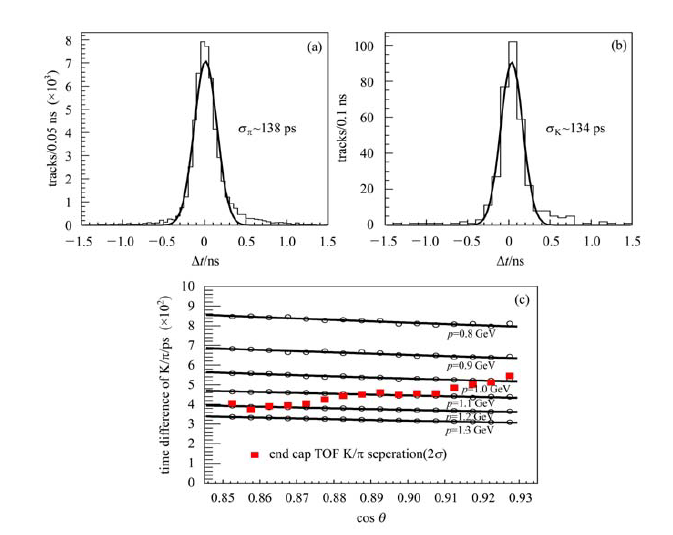
\includegraphics[width=0.9\textwidth]{chap1/end-TOF-PID.png}
  \caption{~1.0~Gev下$\pi$~(a)和~$K$~(b)的时间分辨;(c):端盖~TOF~不同角度下的~$\pi/K$~分辨}
  \label{fig:end-TOF-PID}
\end{figure}

~BESIII~端盖飞行时间探测器采用的是单层的闪烁体结构,以及端盖部分多次散射的影响较大,其本征时间分辨和非本征时间分辨都比较大。

BESIII~谱仪的设计目标是在~$\tau$-粲能区的高精度测量,在这一能区~$J/\psi$~衰变是最主要的物理过程。模拟结果显示,~$J/\psi$~衰变强子动量分布可以达到~1.5~GeV/c,虽然在~0.95~GeV/c以上的强子占的比例较小,但是,对于~BES~物理追求的高精度测量以及稀有衰变事例的研究仍然是非常重要的。因此进一步提高其粒子鉴别能力, 对于提升整个谱仪粒子鉴别能力,完成~BES~物理目标具有重要意义。

测量中性D介子系统的CP破坏和混合参数是~BESIII~的物理目标之一。D介子是唯一没有被测量到~CP~破坏的重味介子。测量D介子混合的黄金衰变道是~$D^0 \to K^- \pi^+$~,~$D^0 \to K^- \pi^+\pi^-\pi^+$~,~$D^+ \to K^- \pi^+\pi^+$~
由于$K$和$\pi$介子的动量分布在~0.8-1.05~GeV,这样我们需要很好的~$\pi/K$~粒子鉴别,要达到较显著的测量结果,要求~$\pi/K$~误鉴别率在~1.05~GeV时要达到~1$\%$~以下。

而~BESIII~目前的端盖~TOF~时间分辨为~140~ps, ~$\pi/K$~的误鉴别率在~1.05~GeV时约为~5$\%$~左右,使得中性D介子的混合参数测量显著性很大程度上下降。由于D介子系统的~CP~破坏很小,粒子物理的标准模型预言~CP~破坏的大小在千分之一左右,要求测量的寻迹系统误差很小,同时也要求~$\pi/K$~的误鉴别应该在~1$\%$~以下。端盖~TOF~的改造不仅改善对带电径迹的粒子鉴别,同时好的飞行时间测量也能提高主漂移室对带电径迹的测量精度,改善寻迹的系统误差,特别是端盖小角度的误差和误鉴别率的改善。当然对于D介子的半轻子衰变和形状因子以及CKM矩阵元Vcs和Vcd的测量,改造后的~TOF~端盖会降低由于粒子误鉴别造成的本底,提高这些物理量的测量精度。 

\section{MRPC~硬件和电子学}
\subsection{端盖MRPC的结构}
升级后的端盖~TOF~采用了~MRPC~技术。利用~MRPC~做成的飞行时间探测器有好的时间分辨,同时又能保证探测效率,有好的粒子鉴别能力,而且价格也便宜。从~MRPC~探测原理出发分析,当带电粒子穿过~MRPC~时,其原初电离的发生雪崩放大现象,这一过程是在多个气隙中同时进行,总的信号等于各个气隙的信号的叠加。因此~MRPC~性能的重要的指标参数是气隙的宽度和数目。采用较小的气隙宽度可以降低工作电压,提高工作稳定性;采用多气隙数目,可以增加带电粒子在气隙中发生雪崩现象的概率,继而可以提高探测效率;可以减小雪崩过程的统计涨落,有利于提高时间分辨。

采用~MRPC~的端盖~TOF~的具体阵列设计如图~\ref{fig:MRPC-TOF}~所示,每层~18~个模块,采用双层结构,通过相邻模块间的交叠可以减少死区,提高探测效率。
\begin{figure}[!h]
  \centering
  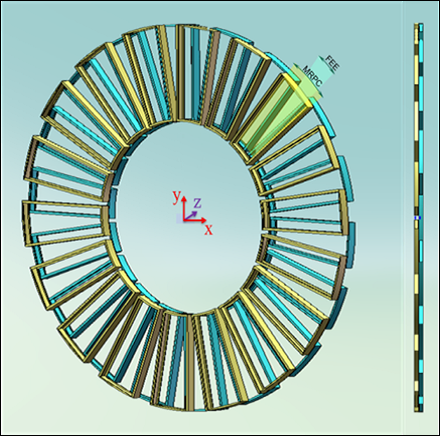
\includegraphics[width=0.5\textwidth]{chap1/MRPC-TOF.png}
  \caption{BESIII/端盖TOF 双层MRPC阵列结构示意图}
  \label{fig:MRPC-TOF}
\end{figure}

每个模块的~PCB~的设计如图~\ref{fig:PCB}~所示。每个模块采用梯形结构,共有~12~个读数条,读数条宽~2.4~cm,相邻读数条之间的距离为~3~mm。读数条最短的是~9.1~cm,最长的是~15.1~cm。每个读数条采用双端读出,共有~24~路读出信号通道。

\begin{figure}[!h]
  \centering
  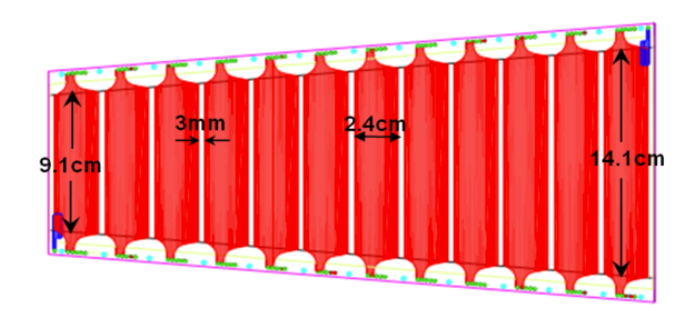
\includegraphics[width=0.9\textwidth]{chap1/PCB.png}
  \caption{MRPC结构示意图}
  \label{fig:PCB}
\end{figure}

MRPC~模型几何结构如图~\ref{fig:MRPC}~所示。模块采用双层堆叠的设计方式,一共有~2*6~个气隙,每个气隙~220~$\mu$m,每个模块的厚度$<$2.4~cm, 双层总厚度$<$5~cm;环状探测器外半径为~844~mm,内半径为~454~mm。
\begin{figure}[!h]
  \centering
  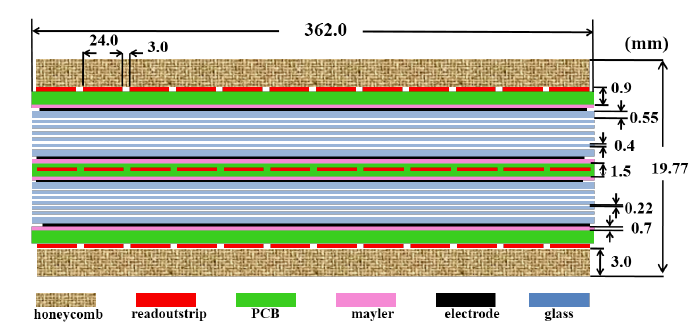
\includegraphics[width=0.9\textwidth]{chap1/MRPC.png}
  \caption{端盖TOF 升级MRPC 的结构图}
  \label{fig:MRPC}
\end{figure}

MRPC~需要工作在气密的环境下,工作气体组分是90$\%$~Freon+5$\%$~S$F_{6}$+5$\%$~iso-$C_{4}H_{10}$。
\subsection{电子学系统}

MRPC~的电子学系统设计方案和电子学系统包含前端放大甄别~FEE(Front end Electronics)模块、飞行时间测量~TDIG(Time to Digital module)插件、提供阈值和电源给~FEE~模块并传输击中信息至触发系统等功能的~CTTP(Coincidence Test Threshold Power module)插件,时钟扇出插件硬件系统和数据获取软件和控制软件系统。

整个系统共~72~个~FEE~模块,FEE~模块采用基于~TOT~技术的~NINO~芯片,每个~FEE~模块含有~4~片~NINO~芯片,产生~24~路LVDS电平的输出信号,共完成~1728~路信号的放大甄别。
MRPC~输出的电荷约为几十fC, 信号脉冲上升时间小于1ns,输出信号电流比较小,必须进行进一步的放大和成形。为了最大程度的利用~MRPC~自身产生的差分信号,~NINO-ASIC~芯片采用差分的输入,全线路的差分信号处理方式。NINO~对输入的信号进行快速放大,同时为了满足过阈时间(TOT)的测量将输入的信号电流转换为了输出的信号宽度。
飞行时间数字化插件~TDIG~。前端电子学输出的信号使用~HPTDC~芯片接收并数字化,并根据数据格式进行打包,经~VME~总线上传至数据获取系统。~NINO~配合~HPTDC~同时测量出信号过阈时间的前沿时间(leading edge)和后沿时间(trailing edge)。其中前沿时间用来定时,结合前沿时间和后沿时间的~TOT~用来修正过阈时间不同引起的时间晃动。
端盖~TOF~电子学系统中,~CTTP~插件共两块,一个~CTTP~插件对应~36~个~FEE~模块。插件的作用是接收~NINO~芯片产生的击中信息,然后通过光纤上传到触发系统;为~NINO~芯片提供阈值电压,电源和测试信号,使芯片正常运行和满足测试需求。~CTTP~插件同时还完成快控制功能。
时钟扇出插件为~TDIG~和~CTTP~插件提供同步时钟信号。

\section{~BESIII~离线数据处理和分析系统}
BESIII~实验开发的一套由软件平台、模拟、刻度、重建和物理分析工具等部分组成的软件系统是为了用来处理和分析~BESIII~离线数据。对探测器和模拟产生的原始数据进行离线处理,生成包含末态粒子各种信息的数据(DST数据)供物理分析使用是它的主要任务,同时连接探测器和物理分析的衔接系统,提供了物理研究所需的各种软件工具。~BESIII~的简化的离线数据处理过程如图~\ref{fig:BESIII-data-flow}~所示。
\begin{figure}[!h]
  \centering
  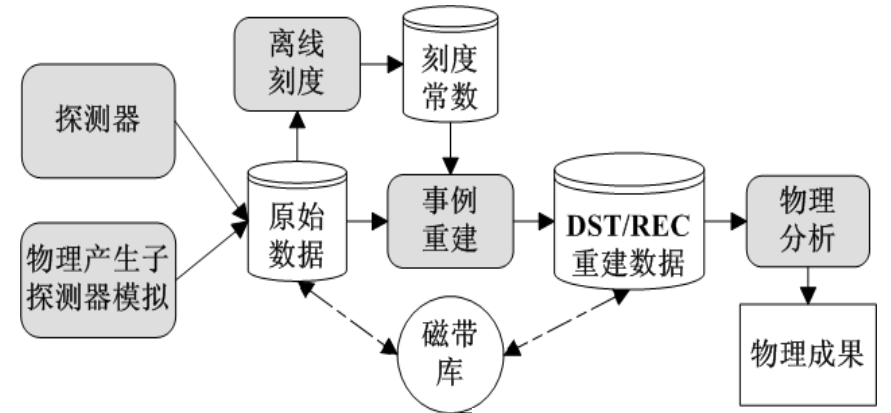
\includegraphics[width=0.9\textwidth]{chap1/BESIII-data-flow.png}
  \caption{简化的BESIII离线数据处理和物理分析过程}
  \label{fig:BESIII-data-flow}
\end{figure}

结合~BESIII~实验的具体需求,选用~cern~的~LHCb~实验开发的通用高能物理实验底层软件框架~GAUDI~~\cite{Barrand:2000}为基础,以C++语言为主要程序语言开发的全新离线数据处理和分析软件平台~\cite{liwd:2006}(BOSS)是~BESIII~离线软件系统的核心部分。

包括离线数据刻度、事例重建、事例分类、MC模拟和物理分析等阶段的离线数据处理的数据管理工具是由BOSS~软件平台提供的。软件平台结合数据处理各阶段的特点和探测器特点的设计出符合不同探测器的数据结构,然后对这些数据采用专门的数据管理服务进行关键。BOSS~软件平台实现动态库的链接机制,可以有效的缩短再编译的时间。软件系统同时采用了如ROOT~\cite{root},CERNLIB~\cite{cern}等国际高能物理实验室的开源软件库和各种软件工具。

图~\ref{fig:BESIII-software}给出了BESIII离线软件平台的整体结构图。软件的核心部分是:模拟、刻度、重建和物理分析算法。
\begin{figure}[!h]
  \centering
  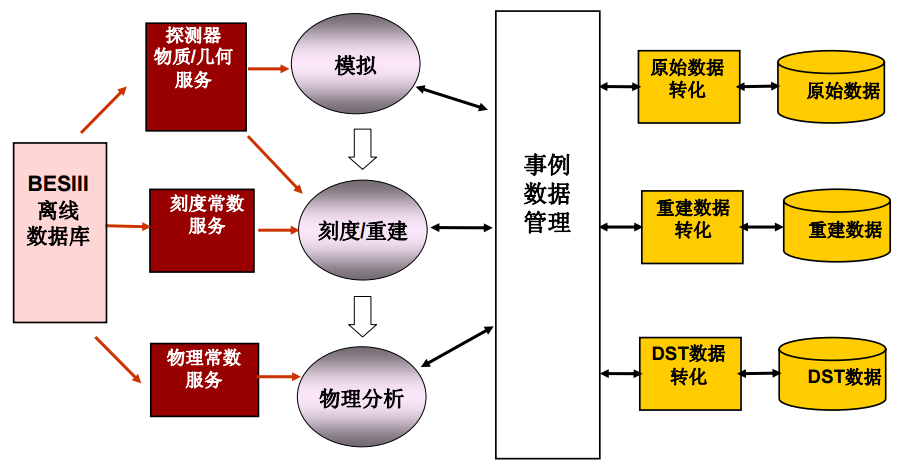
\includegraphics[width=0.9\textwidth]{chap1/BESIII-software.png}
  \caption{BESIII离线软件平台}
  \label{fig:BESIII-software}
\end{figure}

BESIII~数据处理和物理分析软件系统,有超过200个的软件单元。组织和管理这些单元采用的是软件包的形式。BESIII~规范软件开发和发布过程利用的是配置管理工具(Configuration Management Tool,CMT),该工具有一套管理规则和管理工具组成。%【9】

\section{端盖~TOF~数据刻度重建流程}
MDC、EMC、TOF~和~MUC~子系统以及径迹外推和匹配部分组成共同组成~BESIII~离线事例重建软件系统。BEPCII~采用的多束团对撞的机制,BEPCII~的高频时钟为~499.8~MHz,周期为~2~ns,储存环中共有~93~个束团,两个相邻束团之间的时间间隔为~6~ns。BESIII~触发系统的周期为~24~ns,因此在每个触发周期内有~4~个束团对撞,准确的事例起始时间无法由在线系统直接给出。必须通过离线数据分析,通过事例重建,主要是MDC径迹重建,得到最可几事例起始时间。

事例重建系统的一般流程如图~\ref{fig:reconstruction}~。

\begin{figure}[!h]
  \centering
  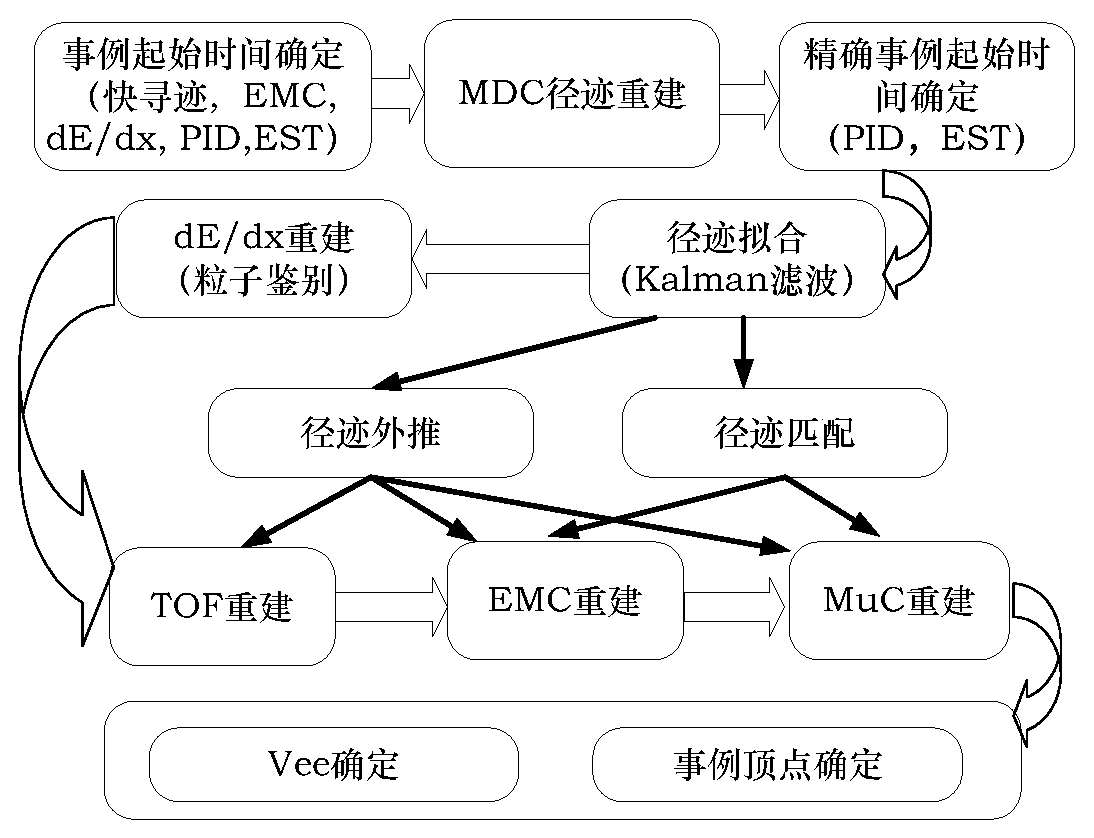
\includegraphics[width=0.7\textwidth]{chap1/reconstruction.eps}
  \caption{BESIII事例重建过程}
  \label{fig:reconstruction}
\end{figure}

\subsection{事例起始时间重建}

前面提到在一个触发周期内有~4~个束团发生对撞,因此准确的事例起始时间无法由在线系统直接给出。事例起始时间需要离线数据重建得到。图~\ref{fig:BESIII-time-system}给出了~BESIII~的时间测量系统。事例的起始时间~$T_{est}$~可以表示为:$T_{est}$=$T_{DCM}$-$T_{ev}$。其中~$T_{est}$~表示事例起始时间,为对撞发生时刻的时间;~$T_{DCM}$~表示~TOF~电子学测量到的原始~TDC~时间,$T_{ev}$~为带电粒子从对撞顶点飞到到给出信号的探测器之间的飞行时间。
\begin{figure}[!h]
  \centering
  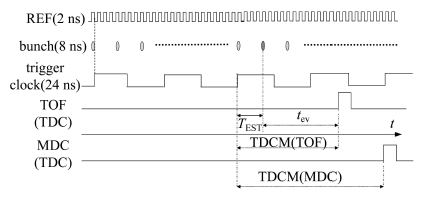
\includegraphics[width=0.6\textwidth]{chap1/BESIII-time-system.png}
  \caption{BESIII事例的时间关系}
  \label{fig:BESIII-time-system}
\end{figure}

图~\ref{fig:Test}~给出了计算事例起始时间~$T_{est}$~的程序流程图。主要包括快重建~\cite{zhangxm:2005}和时间起始时间重建两部分~\cite{max:2007}。在~MDC~快重建和粒子鉴别完成后,$T_{est}$~由~MDC~和~TOF~分别计算得到,具体的计算方法见文献~\cite{Maxiang:2008}。其中~TOF~得到的~$T_{est}$~精确度高。

\begin{figure}[!h]
  \centering
  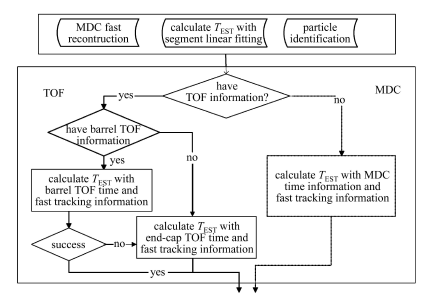
\includegraphics[width=0.6\textwidth]{chap1/Test.png}
  \caption{事例起始时间程序流程图}
  \label{fig:Test}
\end{figure}
\subsection{主漂移室的径迹外推}

~BESIII~主漂移室重建径迹的外推算法,利用小步长外推提供了主漂移室中的带电径迹外推到外部飞行时间探测器,电磁量能器等其他子探测器上的预期径迹信息。算法在外推的过程中充分考虑了带电径迹在磁场中的偏转情况以及带电粒子与探测器物质发生相互作用引起的电离能损等效应, 计算径迹参数的参数误差矩阵时考虑了库仑多次散射效应的影响。

在考虑带电粒子的磁场偏转,以及电离能损的情况下,小步长外推是比较精确的计算径迹的预期参数的一个常用方法。此方法认为径迹可以近似为螺旋线, 在每个小步长外推结束时,从带电粒子的动量中减去该步长的电离能损,之后再进行下一个小步外推,如此直到推至要求的位置~\cite{wangll:2014}。
具体径迹外推程序~TrkExtAlg~流程图见图~\ref{fig:TrkExtAlg}。

\begin{figure}[!h]
  \centering
  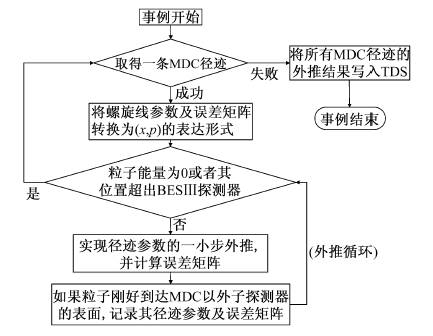
\includegraphics[width=0.6\textwidth]{chap1/TrkExtAlg.png}
  \caption{径迹外推算法的实现流程图}
  \label{fig:TrkExtAlg}
\end{figure}

\subsection{飞行时间探测器的重建}
TOF~离线数据重建流程如图~\ref{fig:TOF-res}~所示。
TOF~电子学系统给出~TOF~的时间信号和幅度信号。MDC~重建和~KalmanFilter~径迹拟合得到带电径迹的动量和径迹长度等信息~\cite{wulh2007}~\cite{wangjk2009},进而计算出粒子飞行的预期时间,径迹外推给出击中~TOF~的位置信息~\cite{wangll:2014},事例起始时间算法~\cite{Maxiang:2008}给出~$t_{0}$~信息,利用这些信息结合刻度得到的刻度常数完成~TOF~的离线数据重建。
\begin{figure}[!h]
  \centering
  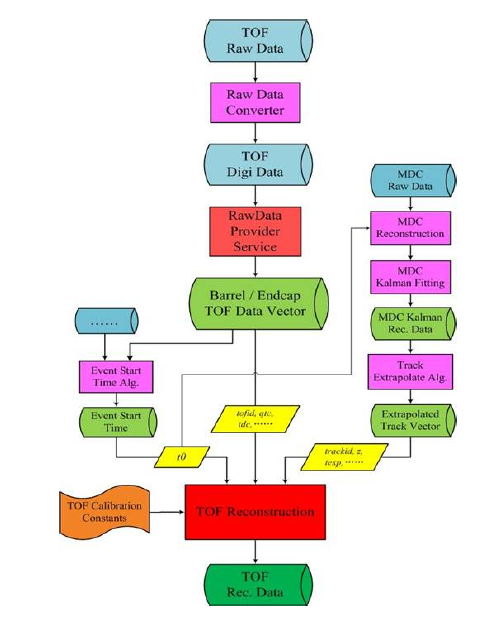
\includegraphics[width=0.6\textwidth]{chap1/TOF-res.png}
  \caption{TOF的离线数据重建过程}
  \label{fig:TOF-res}
\end{figure}

\section{原始数据分布}
图~\ref{fig:digicheck-endcapLeading-east-endcap-histogram}~给出了MRPC端盖TOF的原始的TDC的信息。
\begin{figure}[!h]
  \centering
  \includegraphics[width=0.75\textwidth]{chap1/digicheck-endcapLeading-east-endcap-histogram.eps}
  \caption{原始的TDC}
  \label{fig:digicheck-endcapLeading-east-endcap-histogram}
\end{figure}

图~\ref{fig:T and Q}~给出了~T-Q~匹配后~MRPC~端盖~TOF~的原始的时间和过阈时间的分布。
\begin{figure}[!h]
%\hfill
\begin{minipage}{0.48\linewidth}
  \centerline{ \centering 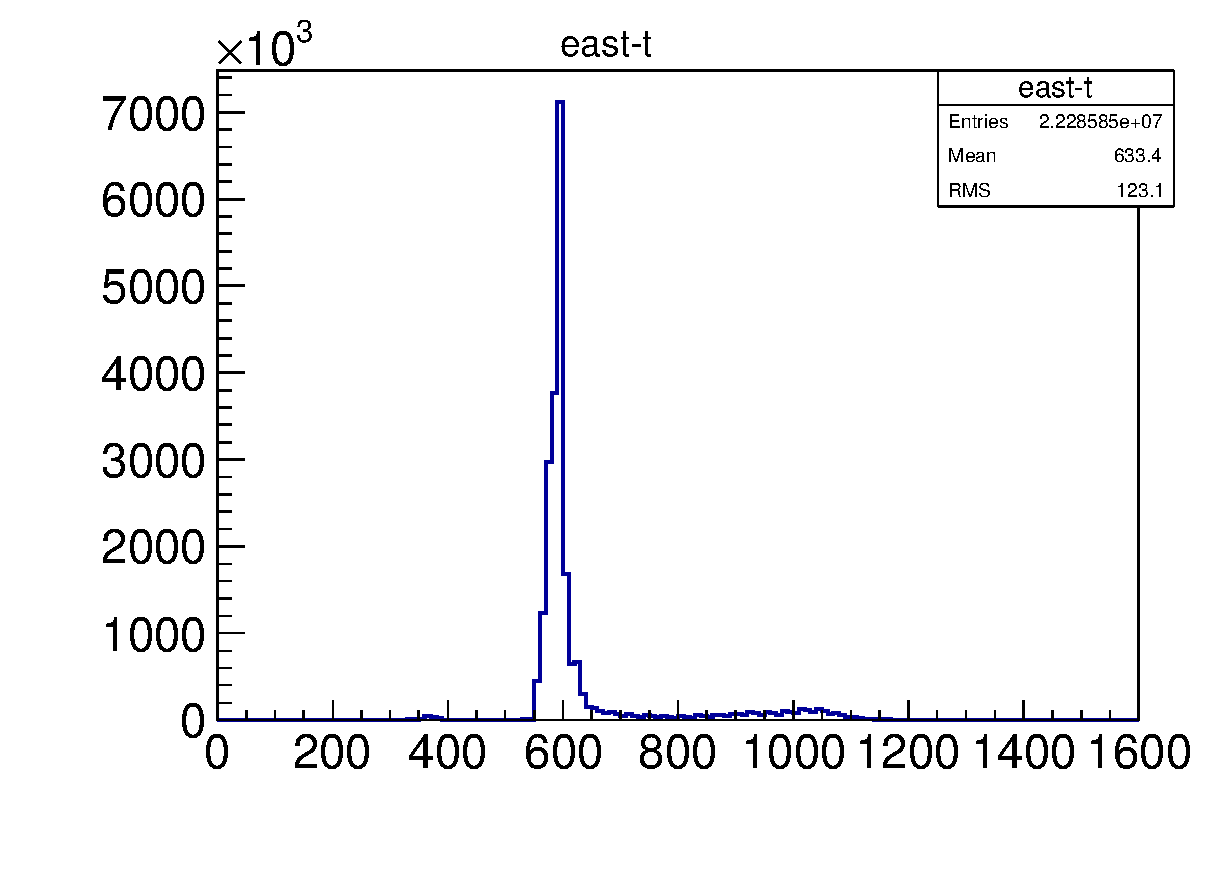
\includegraphics[width=0.75\textwidth]{chap1/endcapcheck-east-t-histogram.eps}}
  \centerline{(a) 东端的原始时间}
  \centerline{\label{fig:endcapcheck-east-t-histogram}}
\end{minipage}
%\hfill
\begin{minipage}{0.48\linewidth}
  \centerline{ \centering 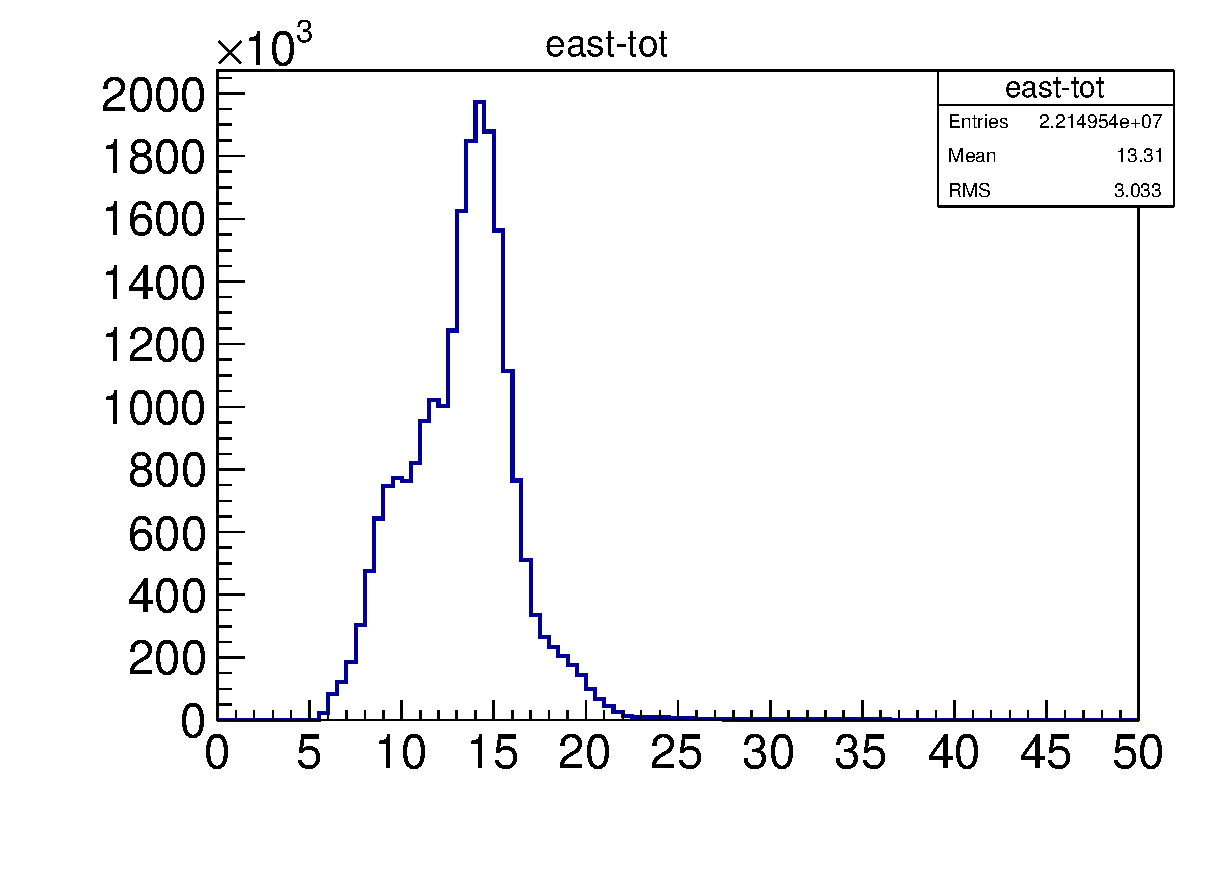
\includegraphics[width=0.75\textwidth]{chap1/endcapcheck-east-tot-histogram.eps}}
  \centerline{(b) 东端的原始TOT}
  \centerline{\label{fig:endcapcheck-east-tot-histogram}}
\end{minipage}
\vfill
%\hfill
\begin{minipage}{0.48\linewidth}
  \centerline{ \centering  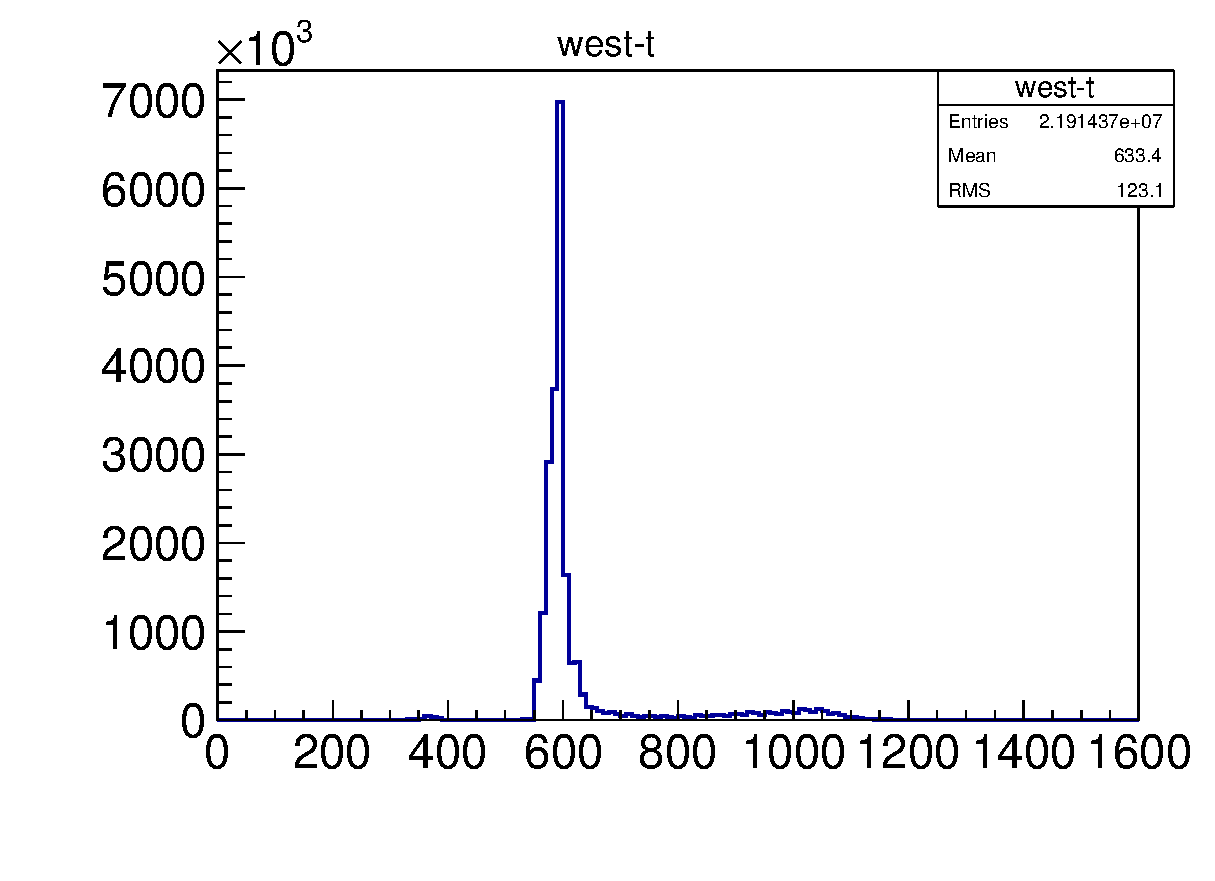
\includegraphics[width=0.75\textwidth]{chap1/endcapcheck-west-t-histogram.eps}}
  \centerline{(c) 西端的原始时间}
  \centerline{\label{fig:endcapcheck-west-t-histogram}}
\end{minipage}
%\hfill
\begin{minipage}{0.48\linewidth}
  \centerline{ \centering 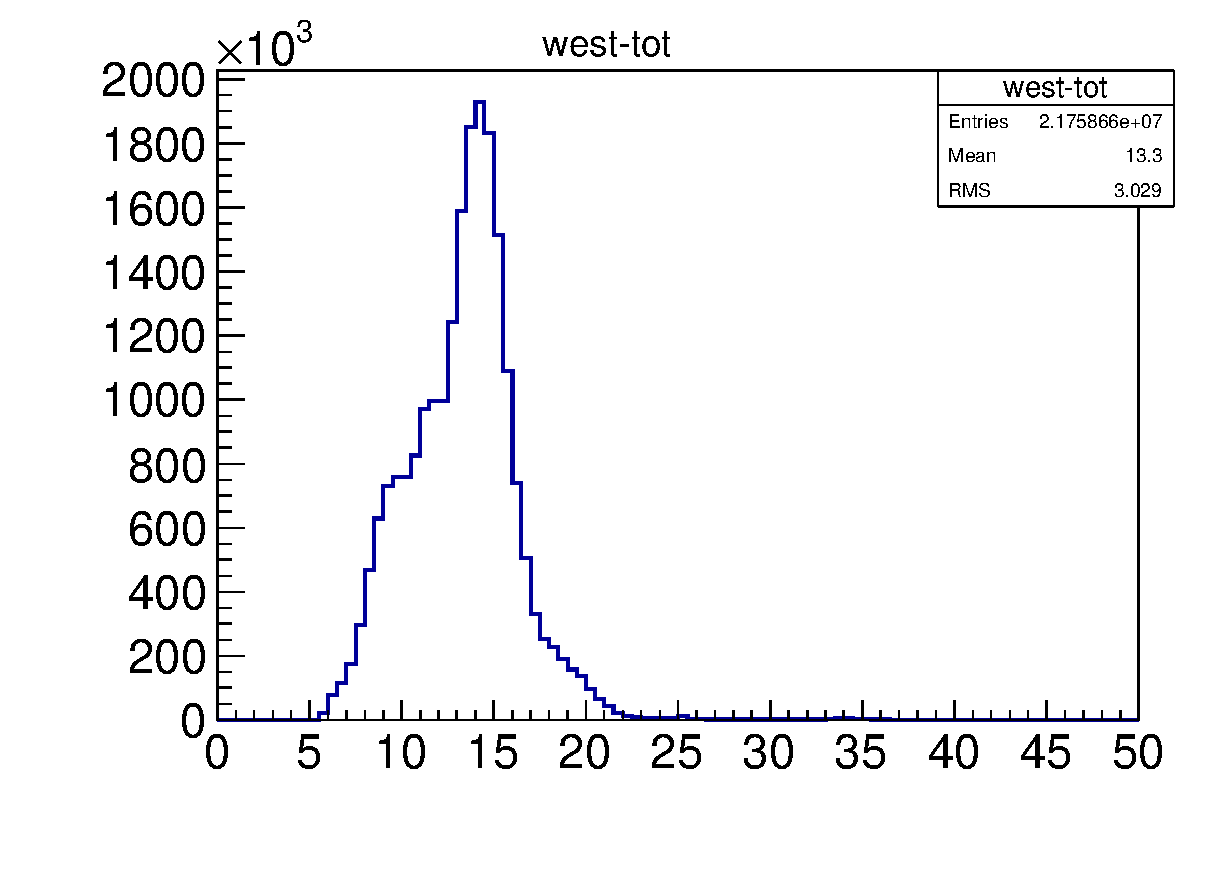
\includegraphics[width=0.75\textwidth]{chap1/endcapcheck-west-tot-histogram.eps}}
  \centerline{(d) 西端的原始TOT}
  \centerline{\label{fig:endcapcheck-west-tot-histogram}}
\end{minipage}
\caption{T-Q匹配后MRPC的原始时间和TOT的分布}
\label{fig:T and Q}
\end{figure}

图~\ref{fig:tofcheck-endcap-est-histogram}~给出了事例起始时间的分布。
\begin{figure}[!h]
  \centering
  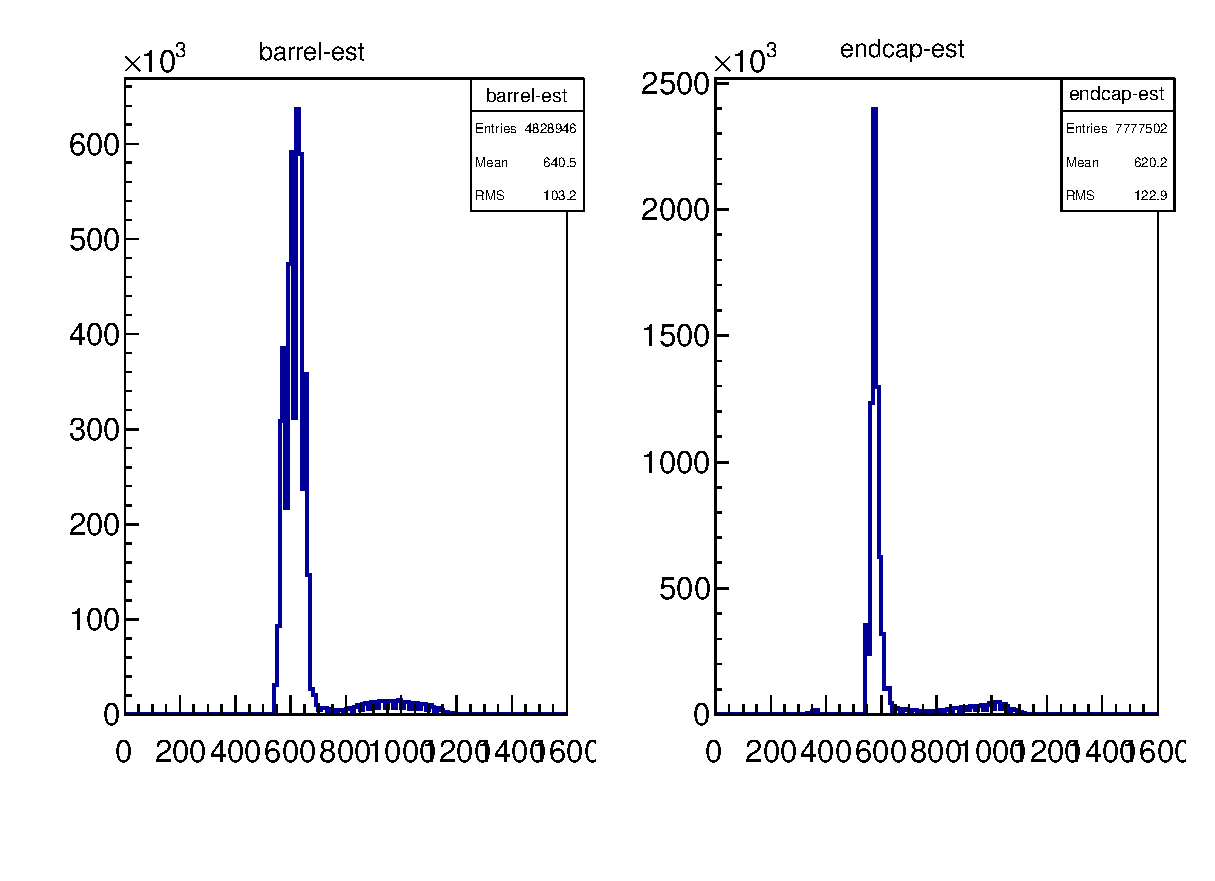
\includegraphics[width=0.9\textwidth]{chap1/tofcheck-endcap-est-histogram.eps}
  \caption{事例起始时间的分布}
  \label{fig:tofcheck-endcap-est-histogram}
\end{figure}

原始测量的时间信号~TDC~包括事例的起始时间~$t_{0}$~,对撞事例从对撞顶点到~TOF~探测器的飞行时间~$t_{tof}$~,信号在读数条的传播时间~$t_{pro}$~,电子学的延迟~$t_{ele}$~,过阈时间的晃动~$t_{time-walk}$~。即:~TDC=$t_{0}$+$t_{tof}$+$t_{pro}$+$_{ele}$+$t_{time-walk}$~,所以飞行时间~$t_{tof}$=TDC-($t_{0}$+$t_{pro}$+$_{ele}$+$t_{time-walk}$)~,其中~TDC~是~TOF~探测器测量到的原始时间信号,对于~MRPC~来讲,采用的双端读数,所以一个事例有两个~TDC~时间信号。~$t_{0}$~由事例起始时间算法给出,~$t_{pro}$~对于~MRPC~来说是信号在对数条的传播时间。这个是刻度的主要内容之一。~$t_{ele}$~是电子学延迟项,是一个常数项。~$t_{time-walk}$~对于~MRPC~来说是~TOT~的晃动。
\section{刻度的重点和难点}
\subsection{MRPC~离线刻度的信息量}
前面已经介绍了~MRPC~直接测量的是时间信号~TDC~,还有过阈时间~TOT~。MRPC~的读数条采用的是双端的读出形式。所以对应一个事例测量的有两个时间信号~TDC1,TDC2;有两个过阈时间~TOT1,TOT2。
在这里定义:
\begin{align}
t_{left}=TDC1-t_{0}
\label{eq:tleft}\\
t_{right}=TDC2-t_{0}
\label{eq:2}
\end{align}
则$t_{left}$和$t_{right}$为事例从对撞点时刻到电子学读出的过阈时间前沿的时刻之间的间隔。包括从对撞点飞行到~MRPC~探测器的飞行时间,信号在读数条中的传播时间,信号在电缆等的传播时间,电子学的时延,过阈时间的晃动等部分。

刻度的目的正是修正除了飞行时间外的其它时间的贡献。其中信号在电缆的传播时间和电子学的时延是常数项,信号在读数条的传播时间是一个依赖击中位置的时间量。过阈时间的晃动是和信号的大小有关的量。

BESIII~系统的坐标定义为:正~Z~轴沿着束流方向,水平向东;正~Y~轴指向天空,竖直向上;正~X~轴取水平向北。取对撞点为坐标原点O(0,0,0)。空间某一点P(x,y,z)的方位角定义为直线OP从正X轴沿逆时针在Z—Y平面投影的角度~$\phi$,在端盖~MRPC~中对应的不同模块的编号和相同模块不同的击中位置(来自径迹外推)。OP的极角定义为OP和正Z轴的夹角~$cos\theta$,在端盖~MRPC~中对应的是读数条的编号。

之前已经介绍了利用~MDC~重建和卡曼滤波径拟合可以得到带电径迹的动量和径迹长度的信息,进而可以求出带电粒子的预期飞行时间~$t_{exp}$。

至此,刻度需要的所有相关量已经介绍完了。包括电子学系统测量的量:初始时间~$t_{left}$,$t_{right}$~(TDC扣除$t_{0}$后的时间在本论文中仍旧称为初始时间),过阈时间~qleft,qright~(测量的两个过阈时间的值在本文中都表示成~qleft,qright~的形式);外推的量:击中位置~zrhit,预期时间~$t_{exp}$,以及模块的编号,读数条的编号。
\subsection{MRPC~离线刻度的时间,过阈时间,击中位置等的原始分布}
图~\ref{fig:some-Diagram}~给出了~MRPC~离线刻度的一些原始的分布。上面的三幅图是原始的时间,过阈时间和击中位置分布的一维图,其中~\ref{fig:left-t}~是原始的时间分布;~\ref{fig:left-q}~是原始的过阈时间的分布,可以明显看出,存在多峰现象;~\ref{fig:left-z}~是击中位置的分布,可以看出事例数随着击中位置是分布均匀的。下面三幅图是原始的时间,过阈时间和击中位置相互关系的二维图,其中~\ref{fig:left-tVSz}~表示时间随击中位置的分布,这个关系近似线性,这是刻度的主要项之一;~\ref{fig:left-tVSq}~表示时间随过阈时间的分布,关系分布复杂,这也是刻度的主要项之一;~\ref{fig:left-qVSz}~表示过阈时间和击中位置的分布。

\begin{figure}[htbp]
\begin{minipage}[t]{0.33\linewidth}
%\centering
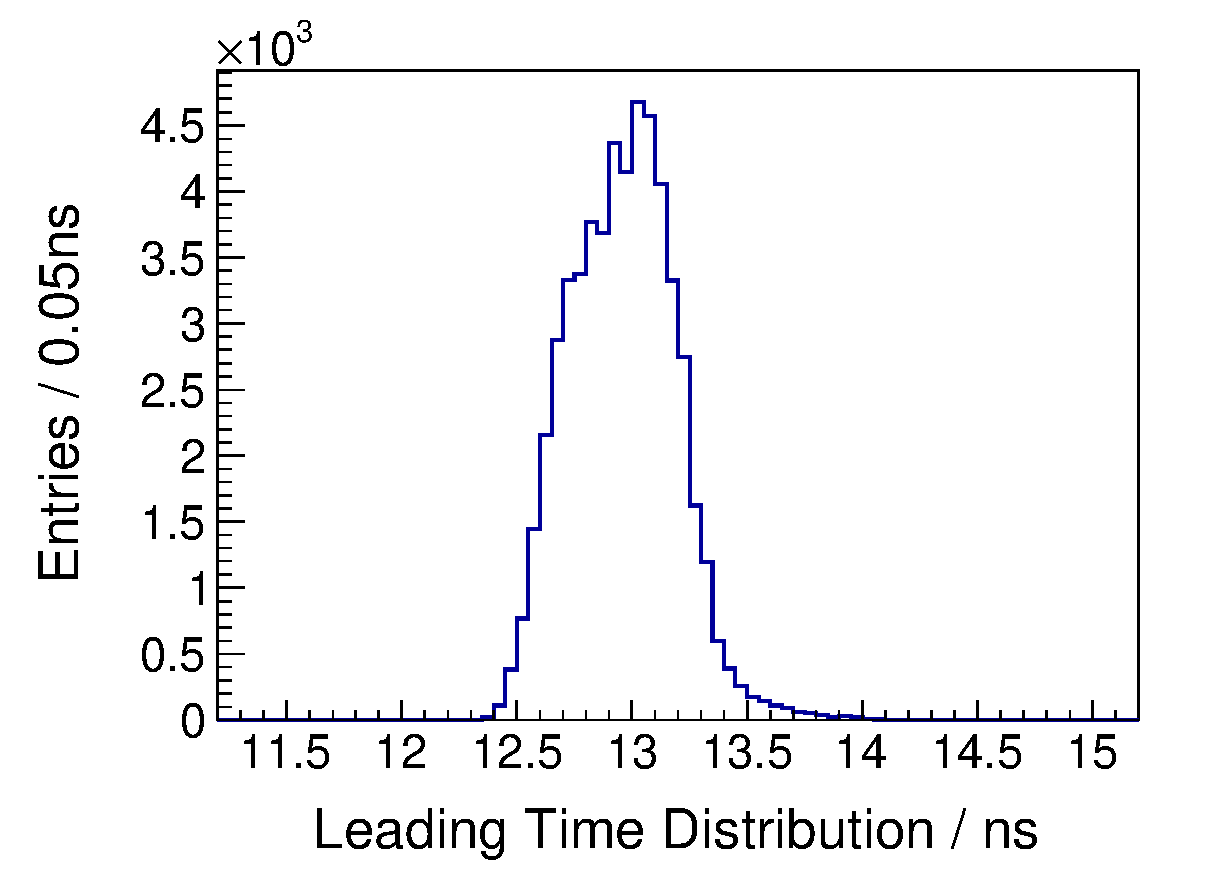
\includegraphics[width=0.9\textwidth]{chap1/left-t.eps}
\subcaption{原始时间的分布}
\label{fig:left-t}
\end{minipage}%
\hfill
\begin{minipage}[t]{0.33\linewidth}
%\centering
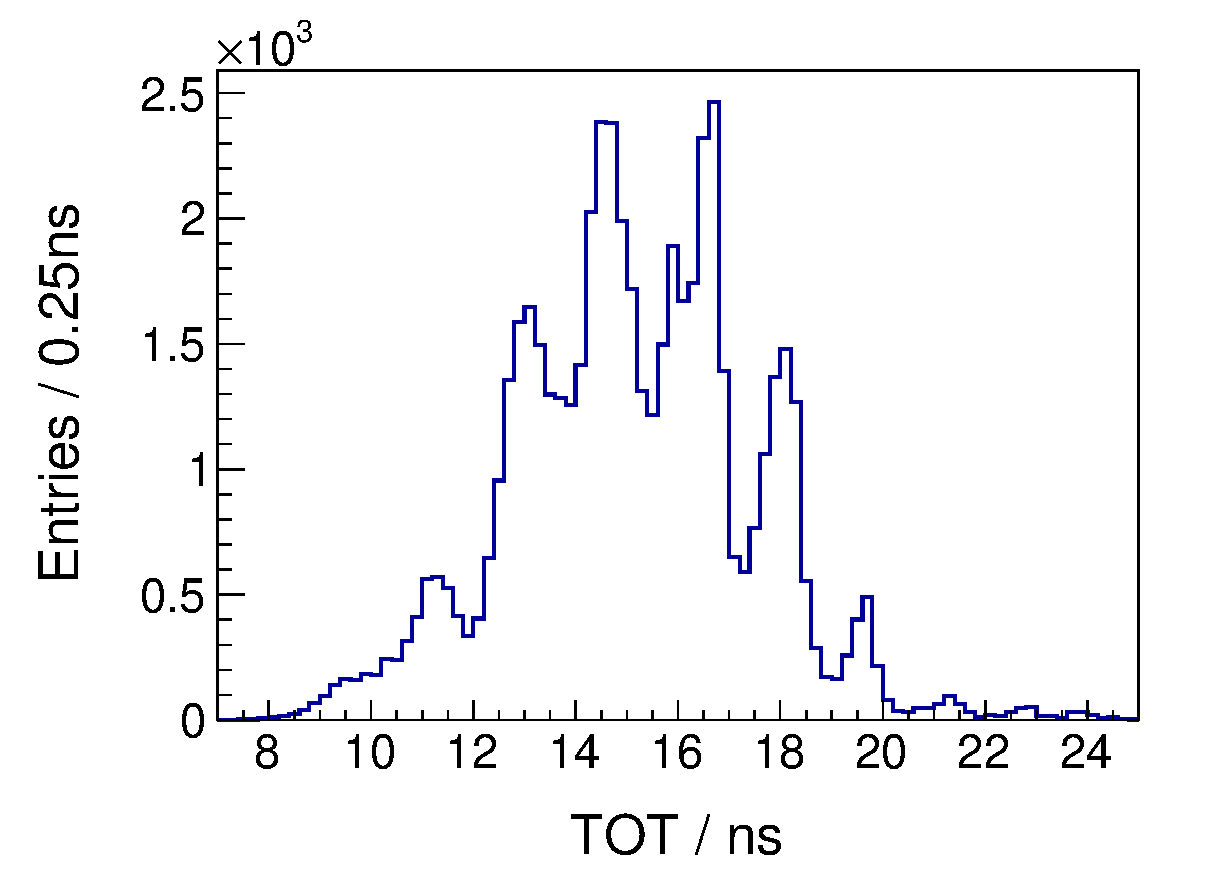
\includegraphics[width=0.9\textwidth]{chap1/left-q.eps}
\subcaption{过阈时间的分布(多峰)}
\label{fig:left-q}
\end{minipage}
\hfill
\begin{minipage}[t]{0.33\linewidth}
%\centering
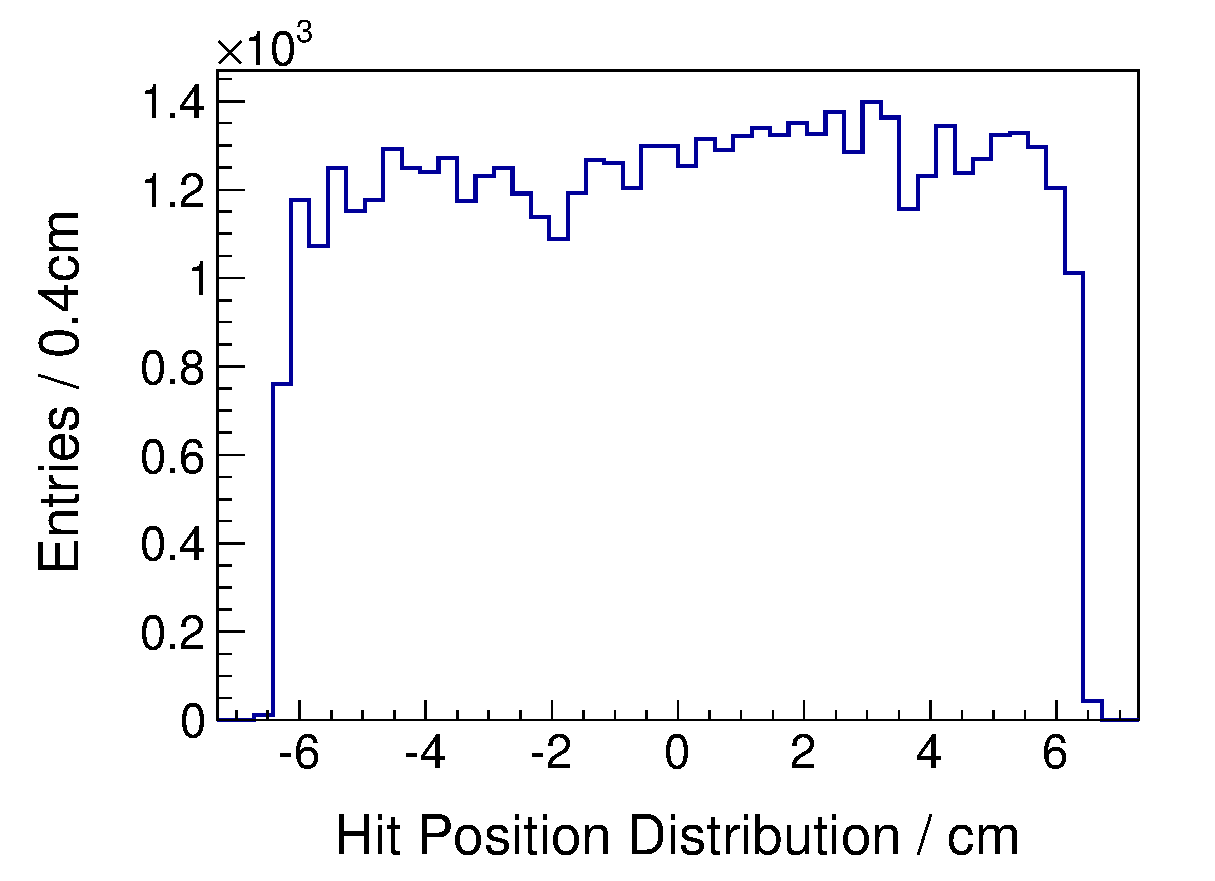
\includegraphics[width=0.9\textwidth]{chap1/left-z.eps}
\subcaption{击中位置的分布}
\label{fig:left-z}
\end{minipage}
\vfill
\begin{minipage}[t]{0.33\linewidth}
%\centering
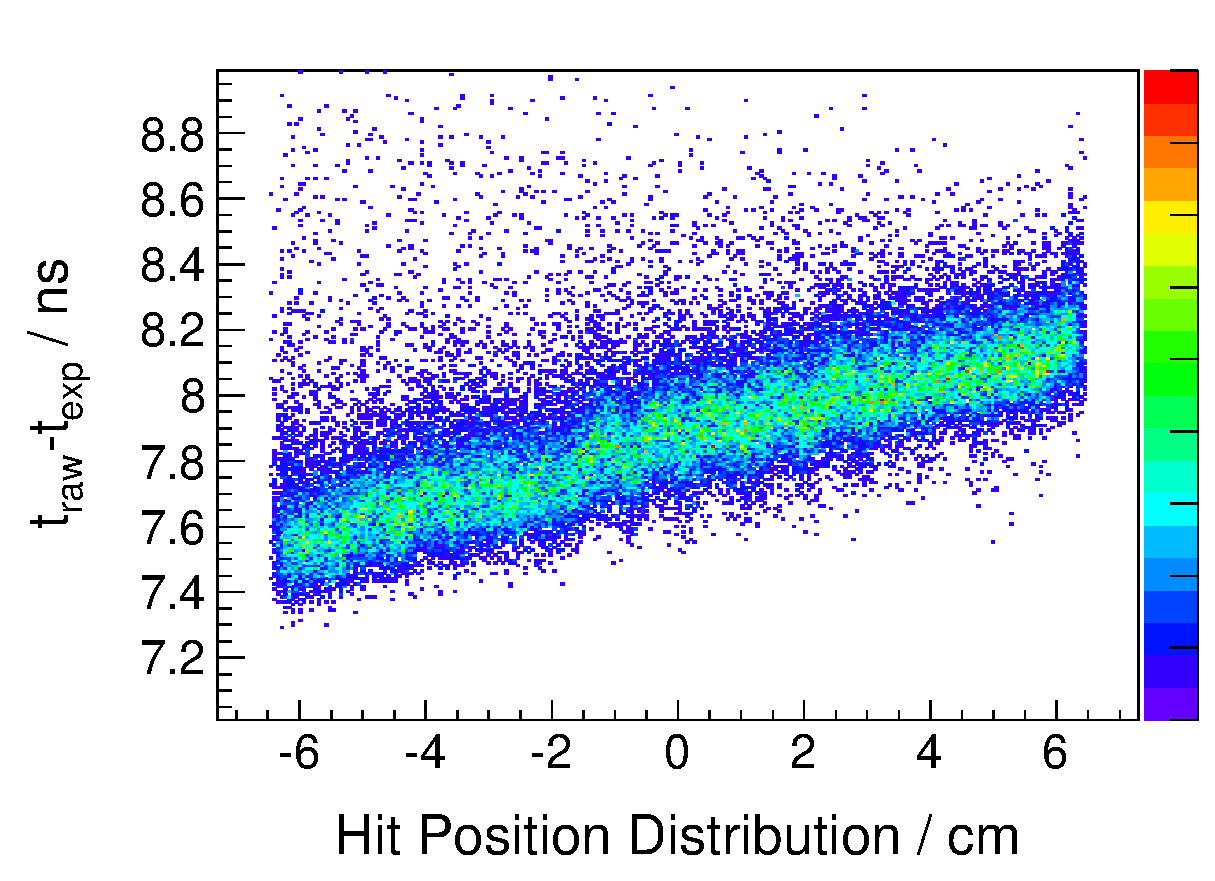
\includegraphics[width=0.9\textwidth]{chap1/left-tVSz.eps}
\subcaption{时间随击中位置的分布}
\label{fig:left-tVSz}
\end{minipage}%
\hfill
\begin{minipage}[t]{0.33\linewidth}
%\centering
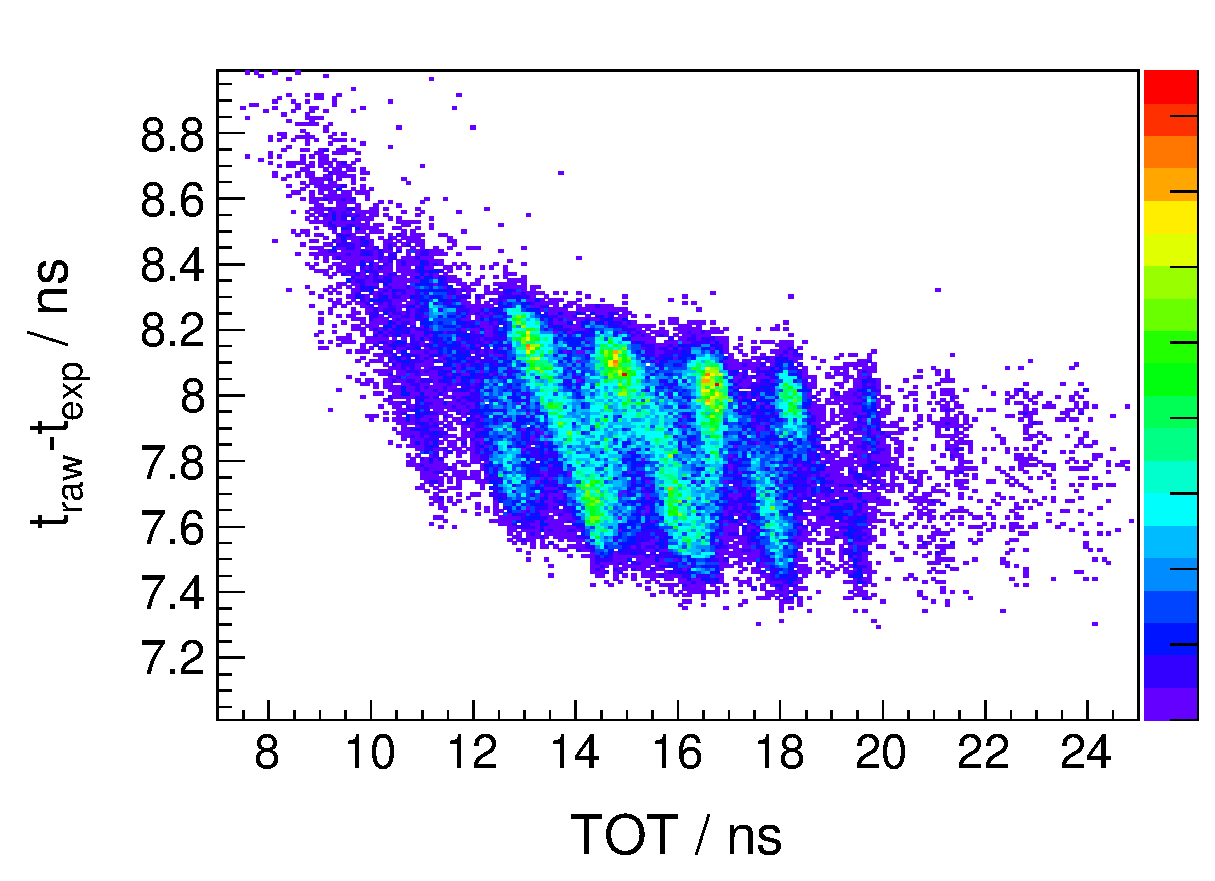
\includegraphics[width=0.9\textwidth]{chap1/left-tVSq.eps}
\subcaption{时间随过阈时间的分布}
\label{fig:left-tVSq}
\end{minipage}
\hfill
\begin{minipage}[t]{0.33\linewidth}
%\centering
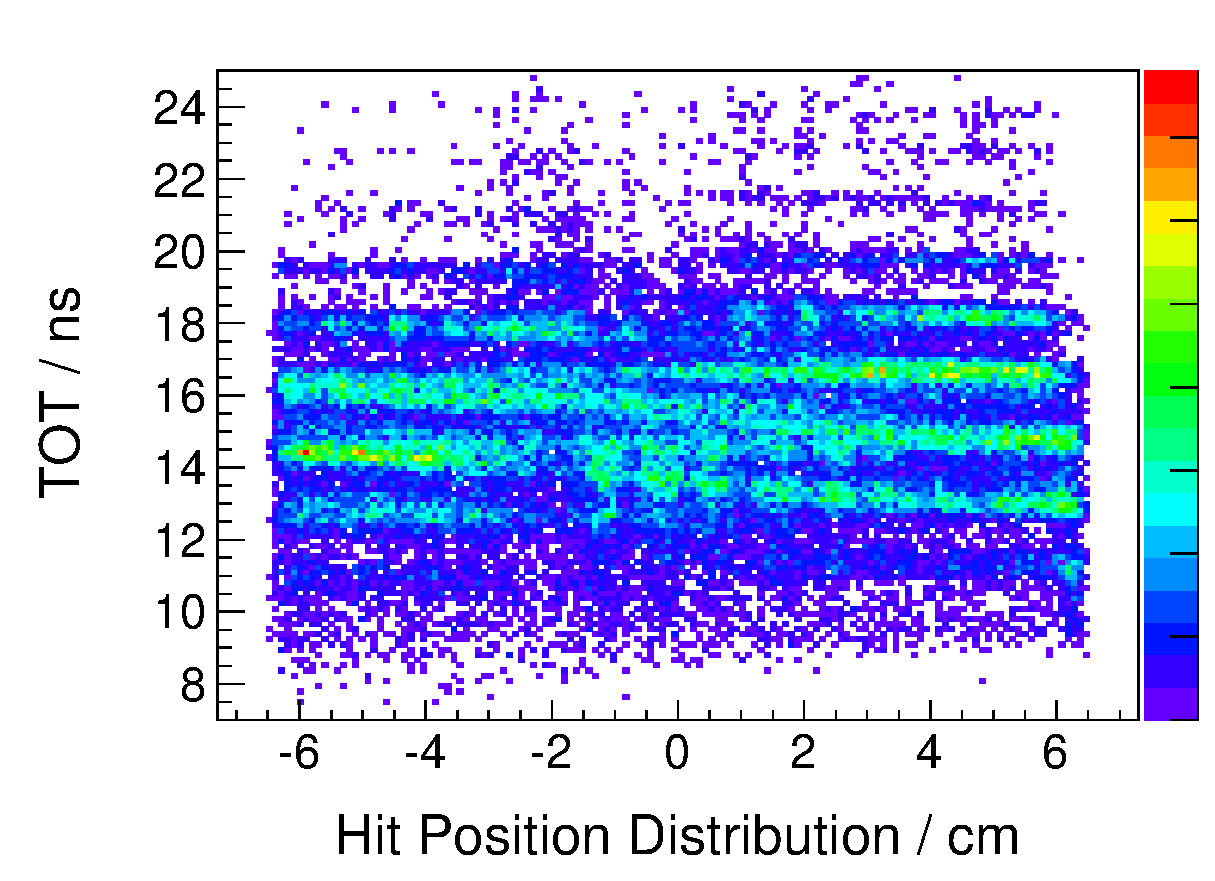
\includegraphics[width=0.9\textwidth]{chap1/left-qVSz.eps}
\subcaption{过阈时间随击中位置的分布}
\label{fig:left-qVSz}
\end{minipage}
\caption{一些原始的分布}
\label{fig:some-Diagram}
\end{figure}

%束团在对撞点发生对撞,产生的次级带电粒子的速度大小和方向在各向都是同性的。
\subsection{过阈时间和反射问题}
刻度的主要内容包括:信号在读数条的传播时间项,过阈时间的修正项。

其中信号在读数条的传播时间和信号在读数条的击中位置以及信号在读数条的等效传播速度有关。对于MRPC的每条读数条而言,长度以及工艺上的差别,导致信号在每个读数条的等效速度不尽相同,因此需要分别对每条读数条进行离线刻度。

信号在读数条的传播时间项如图~\ref{fig:left-tVSz}~所示,近似是一个线性的关系。预估采用低阶多项式即可完成修正。而过阈时间修正项如图~\ref{fig:left-tVSq}~所示,可以看出时间对过阈时间的分布存在折线关系,分布复杂,需要分析这种折线分布背后的产生的机制。采用合适的方式处理这种关系。

\begin{figure}[!h]
\begin{minipage}[!h]{0.5\linewidth}
%\centering
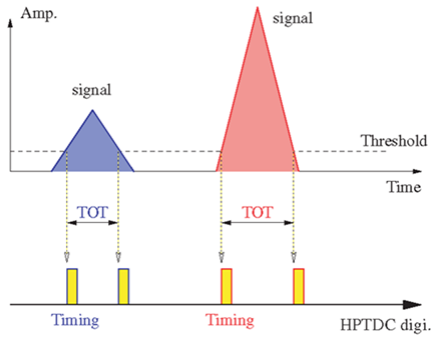
\includegraphics[width=0.8\textwidth]{chap1/TOT.png}
\subcaption{过阈时间~\cite{Shao:2009aa}~}
\label{fig:TOT}
\end{minipage}
\hfill
\begin{minipage}[!h]{0.5\linewidth}
%\centering
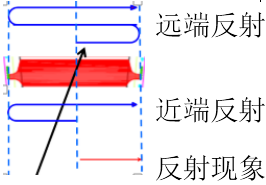
\includegraphics[width=0.9\textwidth]{chap1/reflection.png}
\subcaption{反射问题}
\label{fig:reflection}
\end{minipage}%
\caption{反射问题和过阈时间}
\end{figure}


图~\ref{fig:TOT}~是信号的过阈时间。对于一定的阈值,幅度大小不同的信号,对应的过阈时间不同。信号幅度越大,过阈时间也就越大。
图~\ref{fig:left-q}~中~TOT~的多峰来自于反射。
图~\ref{fig:reflection}~是~MRPC~读数条的反射问题,分为近端反射和远端反射。由于读数条本身较短,反射信号只是比真实信号时间晚不到2ns,这样导致反射信号和原来的真实信号叠加。测量的过阈时间也就变大了。
正是由于过阈时间和反射问题的存在,导致时间对过阈时间的分布复杂。对时间和过阈时间的关系的研究也刻度研究的重点和难点部分。

关于反射和过阈时间有以下结论:
\begin{itemize}
\item{TOT不随击中位置变化}
\item{近端反射是两倍读出条长传播时间。对击中读出条位置没有依赖。}
\item{远端反射依赖击中位置,且与时间依赖关系相反。}
\item{对多次反射的情况,无论近端还是远端反射,相互之间差两倍读出条长的传播时间。}
\end{itemize}

\begin{figure}[!h]
  \centering
  \includegraphics[width=0.9\textwidth]{chap1/TOT-interval.eps}
  \caption{过阈时间的的峰之间的间隔}
  \label{fig:TOT-interval}
\end{figure}
图~\ref{fig:TOT-interval}~表示过阈时间的分布,多峰。两个峰之间的时间间隔是:(19.65ns-11.2ns)/5=1.69ns;

\begin{figure}[!h]
  \centering
  \includegraphics[width=0.9\textwidth]{chap1/TOTvsZ-interval.eps}
  \caption{过阈时间与击中位置图中两个水平线(折线)之间的间隔}
  \label{fig:TOTvsZ-interval}
\end{figure}
图~\ref{fig:TOTvsZ-interval}~表示过阈时间与击中位置的分布。两个水平线之间(近端反射)的时间间隔是:(18.0ns-12.8ns)/3=1.73ns;

读数条编号是~7~的这一条长度是~13~cm,读数条的切角长度是~2.8~cm。信号在读数条传播的等效速度大约是~55~ps/cm(即图~\ref{fig:left-tVSz}~的斜率)。这样信号传播一个读数条长度所需要的时间是:(13+2.8)*55=869ps。传播两倍的读数条长需要的时间是869*2ps=1.738ns。这个值正是对应过阈时间(图~\ref{fig:TOT-interval})之间峰的间隔,和过阈时间与击中位置(图~\ref{fig:TOTvsZ-interval})中两个平行线之间的间隔。

\section{小结}
本章首先介绍了原来的端盖闪烁体~TOF~的时间分辨等性能,由于时间分辨达不到~BESIII~实验高精度测量的要求,端盖~TOF~在~2015~年完成了升级改造,换成了时间分辨更好的~MRPC~探测器。MRPC~探测器作为一种新型的飞行时间探测器,具有时间分辨好,探测效率高,造价便宜等优势。之后介绍了~BESIII~实验的~MRPC~的结构。分东西端盖两部分,各有36个模块。每个模块有12个读数条,采用双端电子学读出信号。BESIII~的离线数据处理和分析系统可以处理包括模拟、刻度、重建和物理分析等一系列的物理问题,其中~BOSS~是整个离线软件的核心。然后介绍了~BESIII~离线数据重建过程,事例起始时间的重建,MDC~的径迹外推,以及~TOF~的离线数据重建过程。最后介绍了~MRPC~端盖TOF的一些原始分布以及刻度的主要内容,MRPC~测量的原始数据是原始的时间和过阈时间。其中原始时间除了包括带电粒子的飞行时间,还有事例起始时间($t_{0}$),信号在读数条内传播的时间,过阈时间的前沿晃动,电缆等的延迟等。这些时间贡献需要刻度修正。其中信号在读数条内的传播时间依赖信号在读数条的有效速度,几乎是一个线性关系。由于反射的原因,导致时间和过阈时间的关系分布复杂。需要采用合适的方式处理。过阈时间的修正也是刻度的重点和难点部分。








  % !TeX root = ../main.tex
% !TEX root = ../main.tex
% -*- root: ../main.tex -*-
% -*- program: pdflatex -*-
\chapter{利用样条插值方法对~MRPC~进行刻度}

~MRPC-TOF~直接测量的信息包括原始的飞行时间和过阈时间(~time-over-threshold~,简称~TOT~)。为了得到精确的飞行时间信息,还需要对时幅游走、过大信号、粒子在对数条上的传播时间,以及在电子学电缆等的时间延迟等因素进行刻度和修正,还要进行离线分析。为了得到良好的时间分辨,必须对不同粒子的样本进行离线的刻度和修正,得到相应的刻度常数,再对原始数据进行重建从而得到飞行时间探测器的性能。
%\begin{comment}
~MRPC-TOF~的离线刻度是通过比较测量时间~$t_{mea}=t_{raw}-t_{0}-t_{cor}$~与带电粒子从对撞顶点到击中~MRPC-TOF~的预期飞行时间~$t_{exp}=L/\beta c$~来比较,其中~$t_{0}$~是事例的起始时间,~$t_{cor}$~是时间的修正项;~c~是真空中的光
速,$\beta=p/\sqrt{p^2+m^2}$是带电粒子的飞行时间,~m~是粒子的质量,飞行长度~L~和动量~P~是通过主漂移室(~MDC~)测量得到的。飞行时间修正项~$t_{cor}$~是过阈时间~TOT~和~Z~向击中位置的函数。
%\end{comment}
对于每一个读数条,每个读出单元定义:
%\begin{equation}
\begin{displaymath}
\chi^2(counter,readout)=\sum\limits_{event}(t_{mea}-t_{exp})^2
\end{displaymath}
%\end{equation}
通过分析大量的事例样本,进行反复迭代,利用最小~$\chi^2$~方法,刻度常数项可以通过~$\partial\chi^2/\partial P_{i}=0$~得到。在重建中,利用刻度得到的刻度常数对原始的飞行时间信息进行重建,就可以得到经过刻度修正得到的飞行时间信息。

STAR~实验MRPC采用的是样条插值(~spline Fit~)刻度的方法。因此本文也对~BESIII~的~MRPC~进行了样条插值方法的研究。
本章主要介绍样条插值方法。分两部分介绍:先对~TOT~进行插值,之后对击中位置~Z~修正;先对击中位置~Z~进行修正,之后对~TOT~进行插值。并进行了一定的结果比较,发现先修正~Z~,然后对~TOT~进行插值的结果比另一种方法好。

样条插值方法优点:光滑性好,且低阶就能拟合的很好。高能所集群下的~root~中有关于~TSpline~的类包,可以利用它完成样条插值的拟合。

本章数据选用的是~160524-160530~这期间~BESIII~对撞数据中的~Bhabha~事例。选用~Bhabha~事例是因为它事例量大,易于挑选,纯度高,适合做刻度样本。

%%%%%%%%%%%%%%%%%%%%%%%%%%%%%%%%%%%%%%%%%%%%%%%%%%%%%%%%%%%%%%%%%%%%%%%%%%%%%%
\section{修正~Z~前进行插值}
%%%%%%%%%%%%%%%%%%%%%%%%%%%%%%%%%%%%%%%%%%%%%%%%%%%%%%%%%%%%%%%%%%%%%%%%%%%%%%

本节以挑选的~Bhabha~事例中击中位置在~MRPC~中模块编号为~55~,对数条编号为~7~这一个对数条为例。具体做法,就是先对~TOT~进行插值修正,之后对得到的结果再次对~Z~进行修正得到最终的时间分辨等刻度信息。
\subsection{等事例数分~bin~拟合}
\begin{itemize}
    \item 以TOT的大小为度量对所选的事例数进行等事例数分~bin~
    \item 对于每个~bin~区间,进行拟合
    \item 对于上一步得到的~mean~值进行插值,得到插值的刻度常数
    \item 利用上一步得到的刻度常数,对时间信息进行修正 
\end{itemize}
等事例数分~bin~的原因是时间随~TOT~的分布是不均匀的。在小~q~(声明:以下所有出现~q~都等同于~TOT~)和大~q~部分事例数很少,如果采用等区间分~bin~的话,会出现比较大的误差棒。分~bin~完成后,发现一个~bin~内时间有两个峰值。图~\ref{fig:ScatterDiagram}~是时间对~TOT~的分布,图~\ref{fig:cutScatterDiagram}~是图~\ref{fig:ScatterDiagram}~截取的一部分。

\begin{figure}[htbp]
\begin{minipage}[t]{0.5\linewidth}
%\centering
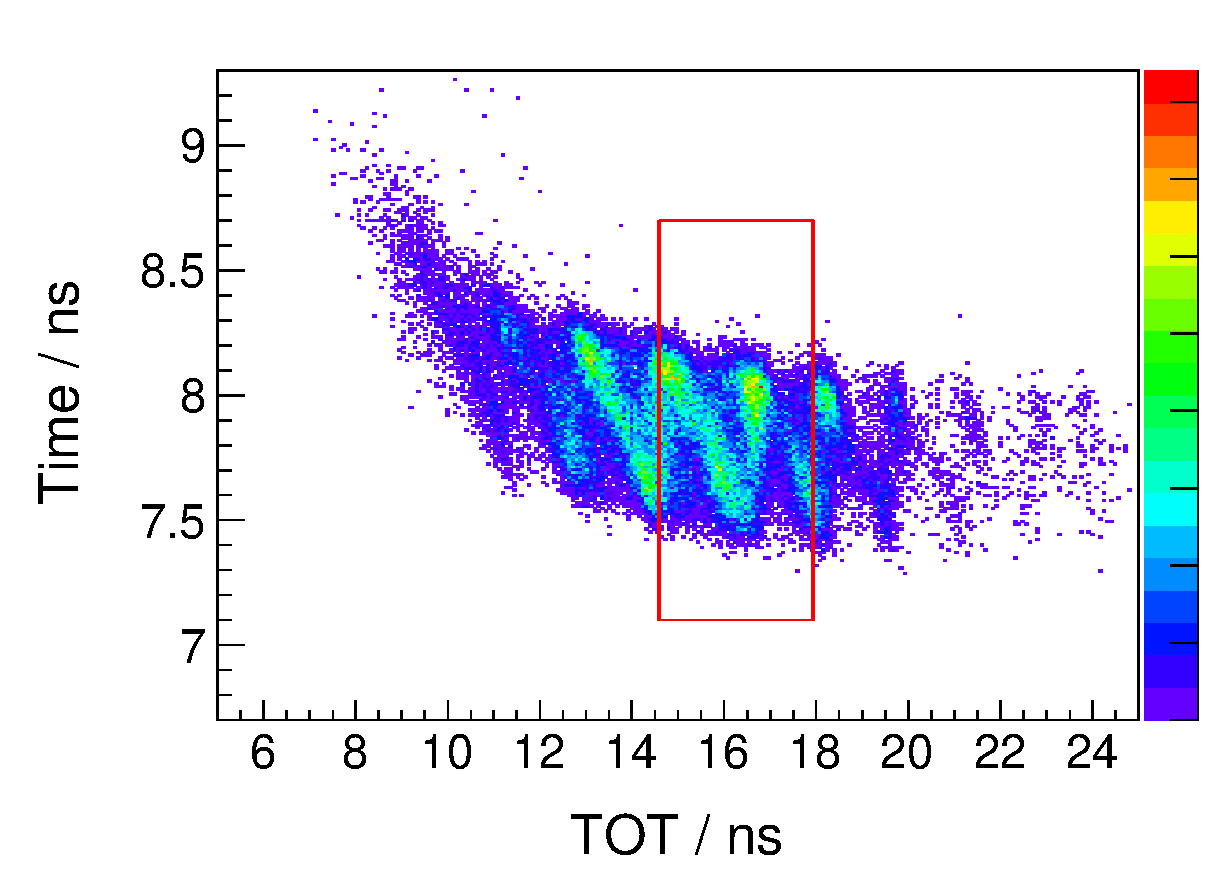
\includegraphics[width=0.9\textwidth]{chap2/ScatterDiagram.eps}
\subcaption{时间对TOT的分布}
\label{fig:ScatterDiagram}
\end{minipage}%
\hfill
\begin{minipage}[t]{0.5\linewidth}
%\centering
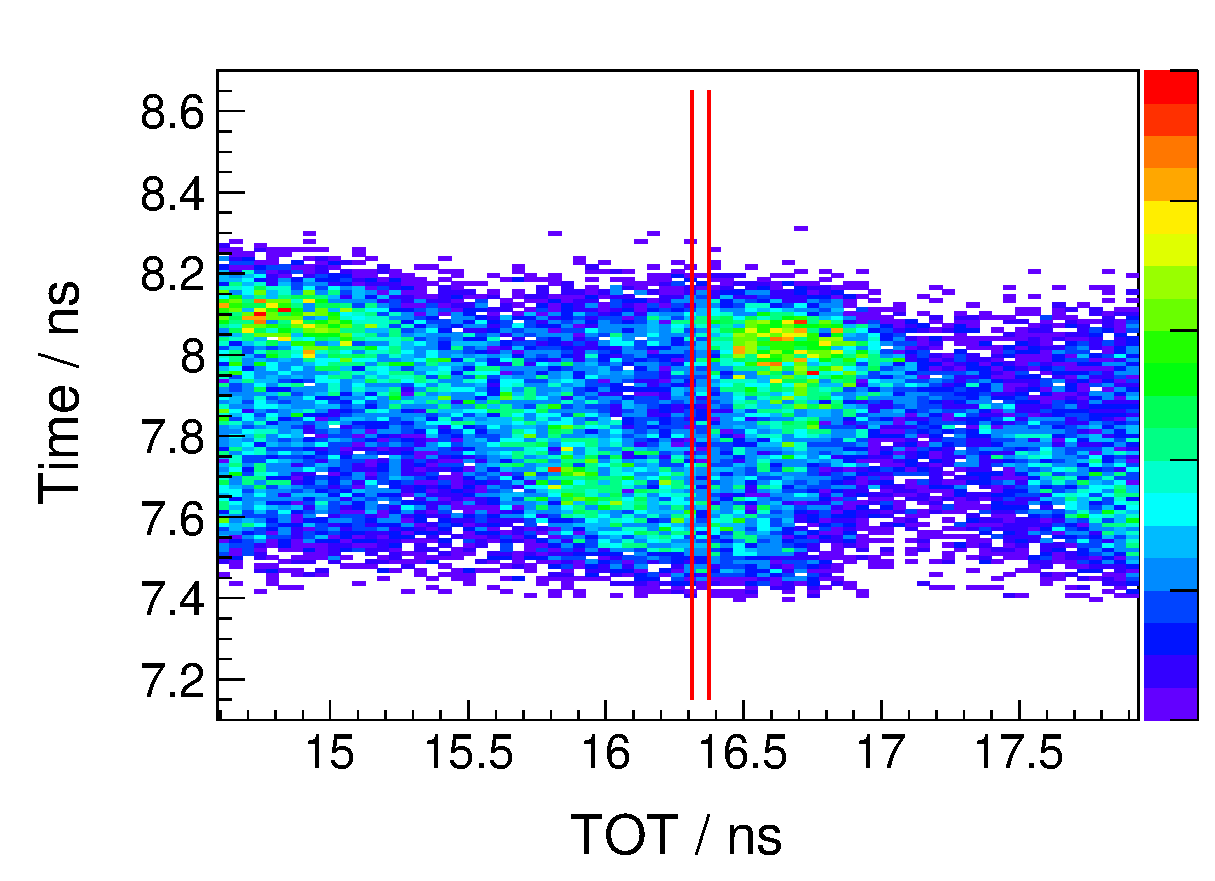
\includegraphics[width=0.9\textwidth]{chap2/cutScatterDiagram.eps}
\subcaption{截取时间对TOT的分布}
\label{fig:cutScatterDiagram}
\end{minipage}
\caption{时间对TOT的分布}
%\label{fig:Diagram}
\end{figure}

\begin{figure}[htbp]
\centering
\includegraphics[width=0.5\textwidth]{chap2/onebinTime.eps}
\caption{截取一个bin的时间分布}
\label{fig:onebinTime}
\end{figure}

图~\ref{fig:onebinTime}~是一个bin内的时间分布,可以明显看出具有双峰。对此,我没有办法在一个区间内得到一个合适的中心值。

\subsection{两个高斯拟合和单个高斯拟合}

图~\ref{fig:double-ScatterDiagram}~,~\ref{fig:single-ScatterDiagram}~分布是对每个~bin~用两个高斯和一个高斯函数拟合后得到的中心值的分布

\begin{figure}[!h]
\begin{minipage}[!h]{0.5\linewidth}
%\centering
\includegraphics[width=0.95\textwidth]{chap2/double-ScatterDiagram.eps}
\subcaption{两个高斯拟合后的graph}
\label{fig:double-ScatterDiagram}
\end{minipage}%
\hfill
\begin{minipage}[!h]{0.5\linewidth}
%\centering
\includegraphics[width=0.95\textwidth]{chap2/single-ScatterDiagram.eps}
\subcaption{一个高斯拟合后的graph图}
\label{fig:single-ScatterDiagram}
\end{minipage}
\caption{高斯拟合后的graph}
\end{figure}

图~\ref{fig:double-leftspline}~第一种做法的样条插值曲线,每个~bin~的时间的中心值取那个比例高的。图~\ref{fig:single-leftspline}~第二种做法的样条插值曲线。可以看出,样条曲线已经把之前graph点的趋势拟合了。

\begin{figure}[!h]
\begin{minipage}[!h]{0.5\linewidth}
%\centering
\includegraphics[width=0.95\textwidth]{chap2/double-leftspline.eps}
\subcaption{两个高斯拟合得到的中心值的样条插值}
\label{fig:double-leftspline}
\end{minipage}%
\hfill
\begin{minipage}[!h]{0.5\linewidth}
%\centering
\includegraphics[width=0.95\textwidth]{chap2/single-leftspline.eps}
\subcaption{一个高斯拟合得到的中心值的样条插值}
\label{fig:single-leftspline}
\end{minipage}
\caption{样条插值}
\end{figure}

\subsection{~Z~的修正}
不管上述的哪种方法,插值修正完~TOT~后,时间随~Z~的分布都还有依赖,对此进行一个~Z~项的修正,然后得到时间分辨。图~\ref{fig:double-leftspline}~第一种做法得到的时间分辨,为~160ps~;图~\ref{fig:single-leftspline}~第二种做法得到的时间分辨,为~92ps~。这个结果和下一节先修正~Z~,后修正~TOT~的结果相比,差别很大。

分析原因:~TOT~的多峰来自反射。一次反射内,时间对~TOT~的依赖近似线性关系,样条插值的光滑性决定不能完全描述这种关系。
\begin{figure}[!h]
\begin{minipage}[!h]{0.5\linewidth}
%\centering
\includegraphics[width=0.8\textwidth]{chap2/double-resolutiongauss.eps}
\subcaption{时间分辨1}
\label{fig:double-resolutiongauss}
\end{minipage}%
\hfill
\begin{minipage}[!h]{0.5\linewidth}
%\centering
\includegraphics[width=0.8\textwidth]{chap2/single-resolutiongauss.eps}
\subcaption{时间分辨2}
\label{fig:single-resolutiongauss}
\end{minipage}
\caption{时间分辨}
\end{figure}

\subsection{反射问题}


图~\ref{fig:TOT}~是信号的过阈时间。对于一定的阈值,幅度大小不同的信号,对应的过阈时间不同。信号幅度越大,过阈时间也就越大。
图~\ref{fig:reflection}~是~MRPC~读数条的反射问题,分为近端反射和远端反射。由于读数条本身较短,反射信号只是比真实信号时间晚不到1ns,这样导致反射信号和原来的真实信号叠加。测量的~TOT~也就变大了。
正是由于过阈时间和反射问题的存在,导致时间对~TOT~的分布复杂。对时间和~TOT~的关系的研究也刻度研究的重点和难点部分。

\begin{figure}[!h]
\begin{minipage}[!h]{0.5\linewidth}
%\centering
\includegraphics[width=0.8\textwidth]{chap2/TOT.png}
\subcaption{过阈时间~\cite{Shao:2009aa}~}
\label{fig:TOT}
\end{minipage}
\hfill
\begin{minipage}[!h]{0.5\linewidth}
%\centering
\includegraphics[width=0.9\textwidth]{chap2/reflection.png}
\subcaption{反射问题}
\label{fig:reflection}
\end{minipage}%
\caption{反射问题和过阈时间}
\end{figure}


%%%%%%%%%%%%%%%%%%%%%%%%%%%%%%%%%%%%%%%%%%%%%%%%%%%%%%%%%%%%%%%%%%%%%%%%%%%%%%%
\section{修正~Z~后进行插值}
%%%%%%%%%%%%%%%%%%%%%%%%%%%%%%%%%%%%%%%%%%%%%%%%%%%%%%%%%%%%%%%%%%%%%%%%%%%%%%

\subsection{~Z~向的修正后,时间对~TOT~的分布}

图~\ref{fig:q-before}~和图~\ref{fig:q-after}~是~Z~修正前后时间对~TOT~的分布。可以看出,修正完~Z~后时间对~TOT~的折线几乎消失。在此基础上,对~TOT~进行插值拟合。
\begin{figure}[!h]
\begin{minipage}[!h]{0.5\linewidth}
%\centering
\includegraphics[width=0.9\textwidth]{chap2/q-before.eps}
\subcaption{~Z~修正前}
\label{fig:q-before}
\end{minipage}%
\hfill
\begin{minipage}[!h]{0.5\linewidth}
%\centering
\includegraphics[width=0.9\textwidth]{chap2/q-after.eps}
\subcaption{~Z~修正后}
\label{fig:q-after}
\end{minipage}
\caption{~Z~修正前后时间对~TOT~的分布}
\end{figure}

\subsection{插值}

图~\ref{fig:after-left-spline}~是修正完~Z~后对~TOT~的样条插值曲线;图~\ref{fig:resolutiongauss}~是这种方法得到的最终的时间分辨,为~64ps~,比之前先对~TOT~插值修正得到的时间分辨好。
\begin{figure}[!h]
\begin{minipage}[!h]{0.5\linewidth}
%\centering
\includegraphics[width=0.9\textwidth]{chap2/after-left-spline.eps}
\subcaption{~Z~修正后对~TOT~进行插值}
\label{fig:after-left-spline}
\end{minipage}%
\hfill
\begin{minipage}[!h]{0.5\linewidth}
%\centering
\includegraphics[width=0.9\textwidth]{chap2/resolutiongauss.eps}
\subcaption{时间分辨}
\label{fig:resolutiongauss}
\end{minipage}
\caption{~Z~修正后插值}
\end{figure}

这种对比也说明了先对~Z~进行修正,之后再对~TOT~进行修正是正确的。

\section{小结}

本章利用样条插值方法,从几个不同的方法对~MRPC~的刻度方法进行了研究和分析。根据不同的方法得到的时间分辨,修正完后时间对~Z~,时间对~TOT~的分布等比较,得出对于~BESIII~实验的~MRPC~刻度应该先对~Z~进行修正,然后对~Z~进行修正。
插值方法

  % !TeX root = ../main.tex
% !TEX root = ../main.tex
% -*- root: ../main.tex -*-
% -*- program: pdflatex -*-
\chapter{构造公式方法}
\section{Z~的修正}
\subsection{Z~向等区间分~bin~}
\subsection{每个~bin~采用~Nov~公式拟合}
\subsection{对得到的~graph~点采用三阶多项式拟合}
\section{TOT~的修正}
\subsection{尝试各种公式}
\subsection{确定这个主项公式}
\section{小结}










  % !TeX root = ../main.tex
% !TEX root = ../main.tex
% -*- root: ../main.tex -*-
% -*- program: pdflatex -*-
\chapter{双端修正}
上两章主要从插值方法和构造公式入手介绍了对TOF的MRPC的离线数据的刻度方法。研究的主要是单端的刻度。这章将介绍双端刻度方法。

\begin{figure}[!h]
\begin{minipage}[!h]{0.5\linewidth}
%\centering
\includegraphics[width=0.9\textwidth]{chap4/combined-tVSz.eps}
\subcaption{双端时间对~Z~的分布}
\label{fig:combined-tVSz}
\end{minipage}%
\hfill
\begin{minipage}[!h]{0.5\linewidth}
%\centering
\includegraphics[width=0.9\textwidth]{chap4/combined-tVSq.eps}
\subcaption{时间对~TOT~的分布}
\label{fig:combined-tVSq}
\end{minipage}
\caption{双端时间对~Z~和~TOT~的分布}
\end{figure}

图~\ref{fig:combined-tVSz}~和图~\ref{fig:combined-tVSq}~是双端的时间对~Z~和~TOT~的分布。所谓双端指的是两端时间的平均值,~TOT~采用的也是两端~TOT~的平均值。从图中可以看出,双端的时间对~Z~的依赖很小,主要就是时间对~TOT~的依赖关系。而这时的时间对~TOT~的依赖关系和单端修正~Z~后时间对~TOT~的分布很类似。因此对于双端修正,直接对~TOT~修正,采用和单端修正~Z~后处理时间与~TOT~的关系相同的办法。

\section{双端插值方法}
也是先利用插值方法对双端进行修正。
\section{双端构造公式}
\section{双端对~Z~的修正}
为了绕开径迹外推的信息~zrhit~,采用类似的信息(tleft-tright)/2
\section{小结}













  % !TeX root = ../main.tex
% !TEX root = ../main.tex
% -*- root: ../main.tex -*-
% -*- program: pdflatex -*-
\chapter{刻度公式的适用性研究}
前面的三章都是以~MRPC~的模块编号为~55~,读数条的编号为~7~这一条读数条为例进行研究的。在之前的第二章介绍~BESIII~的~TOF-MRPC~的结构时,讲到现在的端盖~MRPC~有东西两部分组成,每部分~36~个模块。每个模块有~12~个读数条。共计~864~个读数条。显然,刻度公式需要对于这~864~个读数条都是适用的。这一章就是探讨刻度公式的适用性的问题。
\section{刻度常数及刻度后的时间分辨}
在第4章和第5章的研究中,对于击中位置的修正采用多项式修正;对于过阈时间的修正,进行了击中公式的比较。其中公式${p_{0}+p_{1}/\sqrt{q}+p_{2}/q}$是拟合比较的一个公式。基于此:这里选用公式如下:

单端:$p_{0}+p_{1}/\sqrt{q}+p_{2}/q+p_{3}*zrhit+p_{4}*zrhit^{2}+p_{5}*zrhit^{3}+p_{6}*zrhit^{4}$

双端:$p_{0}+p_{1}/\sqrt{q}+p_{2}/q+p_{3}*t_{sub}+p_{4}*t_{sub}^{2}+p_{5}*t_{sub}^{3}+p_{6}*t_{sub}^{4}$

其中对于单端:~q~表示的是过阈时间(TOT),~zrhit~表示的是击中位置;对于双端:~q~表示的是双端的是过阈时间的平均值,$t_{sub}$表示的是测量的初始时间差的一半,即($t_{sub}$=$t_{left}$-$t_{right}$)/2,和~zrhit~一样是修正击中位置的量。

%以此为刻度公式,选择2016年5月24日到5月30日的Bhabha事例为刻度样本,在~root~下,配置好刻度重建环境,写好刻度脚本,然后提交到~BESIII~集群上,完成刻度工作。

以此为刻度公式,选择2016年5月24日到5月30日的Bhabha事例为刻度样本,完成刻度工作。

\begin{figure}[!h]
\centering
\includegraphics[width=0.9\textwidth]{chap5/calibration-par.png}
\caption{刻度后截取的两个模块共24条读数条的刻度常数}
\label{fig:calibration-par}
\end{figure}
图~\ref{fig:calibration-par}~给出了单端刻度后的部分读数条的刻度常数。其中第一列表示的是一个行号,对应不同的读数条的编号。第二列表示的是刻度项的常数项,主要在8-9ns之间,之后的两项表示的是和过阈时间相关的刻度常数。最后的四项是和击中位置相关的刻度常数,其中的第一项基本在0.055ns/cm,基本和信号在读数条内的传播速度一致。

图~\ref{fig:calib-res-160524-30}~给出了这一周的数据刻度得到的单端和双端的整体的时间分辨。其中单端的为67ps,双端的为56.6ps。
\begin{figure}[!h]
\centering
\includegraphics[width=0.9\textwidth]{chap5/calib-res-160524-30.eps}
\caption{最终整体的时间分辨}
\label{fig:calib-res-160524-30}
\end{figure}

图~\ref{fig:after-Calibration}~给出了刻度修正后时间对击中位置和过阈时间的分布。其中上面三幅图表示时间和击中位置的分布,分别为两个单端和一个双端;下面三幅图表示时间对过阈时间的分布,分别对应两个单端和一个双端
\begin{figure}[htbp]
\begin{minipage}[t]{0.33\linewidth}
%\centering
\includegraphics[width=0.9\textwidth]{chap5/after-cor-tVSz-left.eps}
\subcaption{单端left刻度后时间对击中位置的分布}
\label{fig:after-cor-tVSz-left}
\end{minipage}%
\hfill
\begin{minipage}[t]{0.33\linewidth}
%\centering
\includegraphics[width=0.9\textwidth]{chap5/after-cor-tVSz-right.eps}
\subcaption{单端right刻度后时间对击中位置的分布}
\label{fig:after-cor-tVSz-right}
\end{minipage}
\hfill
\begin{minipage}[t]{0.33\linewidth}
%\centering
\includegraphics[width=0.9\textwidth]{chap5/after-cor-tVSz-combined.eps}
\subcaption{双端刻度后时间对击中位置的分布}
\label{fig:after-cor-tVSz-combined}
\end{minipage}
\vfill
\begin{minipage}[t]{0.33\linewidth}
%\centering
\includegraphics[width=0.9\textwidth]{chap5/after-cor-tVSq-left.eps}
\subcaption{单端left刻度后时间对过阈时间的分布}
\label{fig:after-cor-tVSq-left}
\end{minipage}%
\hfill
\begin{minipage}[t]{0.33\linewidth}
%\centering
\includegraphics[width=0.9\textwidth]{chap5/after-cor-tVSq-right.eps}
\subcaption{单端right刻度后时间对过阈时间的分布}
\label{fig:after-cor-tVSq-right}
\end{minipage}
\hfill
\begin{minipage}[t]{0.33\linewidth}
%\centering
\includegraphics[width=0.9\textwidth]{chap5/after-cor-tVSq-combined.eps}
\subcaption{双端刻度后时间对过阈时间的分布}
\label{fig:after-cor-tVSq-combined}
\end{minipage}
\caption{刻度修正后时间对击中位置和过阈时间的分布}
\label{fig:after-Calibration}
\end{figure}

\section{刻度算法的稳定性}
对于MRPC刻度而言,一个适合的刻度算法应该能够适用所有模块和所有读数条。这一节就探讨刻度算法的稳定性问题。

图~\ref{fig:calib-res-tofid-combined-160524-30}~给出的时间刻度后时间分辨随MRPC模块的分布,对于每个模块最终的时间采用的是一个高斯拟合,左图是每个模块的时间采用高斯拟合的中心值分布,右图是高斯拟合得到的方差,也就是模块的时间分辨的分布;其中红色的点表示双端结果,蓝色和黑色的点表示单端的结果。时间分辨随着模块的编号分布基本稳定。
\begin{figure}[!h]
\centering
\includegraphics[width=0.9\textwidth]{chap5/calib-res-tofid-combined-160524-30.eps}
\caption{时间分辨随MRPC模块的编号的分布}
\label{fig:calib-res-tofid-combined-160524-30}
\end{figure}

\begin{figure}[!h]
\centering
\includegraphics[width=0.9\textwidth]{chap5/calib-res-strip-combined-160524-30.eps}
\caption{时间分辨随MRPC读数条的编号的分布}
\label{fig:calib-res-strip-combined-160524-30}
\end{figure}
图~\ref{fig:calib-res-strip-combined-160524-30}~给出的时间刻度后时间分辨随MRPC读数条的分布。对于每个读数条的最终时间采用一个高斯拟合,左图是每个读数条的时间采用高斯拟合的中心值分布,右图是高斯拟合得到的方差,也就是模块的时间分辨的分布,其中红色的点表示双端结果,蓝色和黑色的点表示单端的结果。这个分布怎么解释????

\begin{figure}[!h]
\centering
\includegraphics[width=0.9\textwidth]{chap5/tofid55-Par2Sca.eps}
\caption{模块编号为55的双端关于过阈时间刻度项和散点图的关系}
\label{fig:tofid55-Par2Sca}
\end{figure}
图~\ref{fig:tofid55-Par2Sca}~给出了~MRPC~的模块编号为~55~的双端的刻度关于过阈时间项的公式和散点图的关系。可以看出,这个模块~12~个读数条符合的都比较好。说明关于过阈时间的$p_{0}+p_{1}/\sqrt{q}+p_{2}/q$对于整个模块是适用的。

\section{过阈时间和击中位置关联项的研究}
前面研究的都是时间和过阈时间,时间和击中位置之间的关系情况。这一小节主要介绍一下关于过阈时间和击中位置关联项的研究。研究是在本章之前介绍的7项公式基础上添加过阈时间和击中位置关联项,然后刻度,然后比较最终得到的时间分辨,时间分辨随模块的编号的分布和时间分辨随读数条的编号的分布等。主要研究了添加$z/\sqrt{q}+z^{2}/\sqrt{q}$和$z/q+z^{2}/q$的最终结果。
最终得到的分布和不添加这些相关项得到的分布基本无差别。说明,在~7~项公式刻度修正后过阈时间和击中位置之间的关联项的作用很弱。

\begin{table}[h]
    \centering
    \caption{\label{tbl:some-res} 过阈时间和击中位置关联项对时间分辨的影响}
  \footnotesize
    \begin{tabular}{lccc}
        \hline
        公式& 单端left时间分辨(ps)& 单端right时间分辨(ps)& 双端的时间分辨(ps)\\
        \hline
        7项公式& 67.2& 67& 56.6 \\
        7项公式+$z/\sqrt{q}+z^{2}/\sqrt{q}$& 66.7& 66.5& 56.3 \\
        7项公式+$z/q+z^{2}/q$& 66.7& 66.5& 56.3 \\
        \hline
    \end{tabular}
\end{table}

表~\ref{tbl:some-res}~给出了添加关联项后时间分辨的对比情况。可以看出添加的这两种关联项的情况对于最终的时间分辨的影响都是很小的。说明关联比较弱。至于时间随过阈时间,时间随击中位置,以及时间分辨随模块的编号,时间分辨随读数条的编号等的分布变化甚微。

\section{小结}
本章介绍了刻度公式的适用性问题。通过对2016年5月24日到5月30日这一周的数据进行刻度,比较得到的刻度常数的稳定性,刻度得到的时间分辨随着和模块和读数条的分布等情况,确认选用的刻度公式是适用的。在此基础上对过阈时间和击中位置关联项进行了研究,发现它们之间的关联在刻度修正之后比较弱。
%/besfs/groups/cal/tof/guoyx/TofCalib/boss701/TofCalib/final-160524-30/Calib









  % !TeX root = ../main.tex
% !TEX root = ../main.tex
% -*- root: ../main.tex -*-
% -*- program: pdflatex -*-
\chapter{总结}















  % 附录
%  \appendix

  %\include{chapter/chap-req}


%%%%%%%%%%%%%%%%%%%%%%%%%%%%%%
%% 附件部分
%%%%%%%%%%%%%%%%%%%%%%%%%%%%%%
\backmatter
%  \fancyfoot[LE,RO]{\small ~\thepage~}          %页脚为阿拉伯数字的页码,偶数页左端对齐,奇数页右端对齐

  % 参考文献
  % 使用 BibTeX
  \bibliography{tex}
  \nocite{*}
  % 不使用 BibTeX
  % \include{chapter/bib}

  % 发表文章目录
%  \include{chapter/pub}

  % 个人简历
  % !TeX root = ../main.tex
% !TEX root = ../main.tex
% -*- root: ../main.tex -*-
% -*- program: pdflatex -*-
\begin{resume}

\begin{resumesection}{基本情况}
郭迎晓,男,河南省新乡市人,1991 年~5 月出生,未婚,
中国科学院高能物理研究所在读硕士研究生。
\end{resumesection}

\begin{resumelist}{教育状况}


2010~年~9~月至~2014~年~6~月,湘潭大学,本科,专业:物理学。

2014~年~9~月至~2017~年~7~月,中国科学院高能物理研究所, 硕士,专业:计算机技术。
\end{resumelist}

\begin{resumelist}{工作经历}
无。
\end{resumelist}

\begin{resumelist}{研究兴趣}
TOF刻度。
\end{resumelist}

\begin{resumelist}{联系方式}
通讯地址:北京市石景山区玉泉路~19~号乙 中国科学院高能物理研究所

邮编:100049

E-mail: guoyingxiao@ihep.ac.cn
\end{resumelist}

\end{resume}


  % 致谢
  % !TeX root = ../main.tex
% !TEX root = ../main.tex
% -*- root: ../main.tex -*-
% -*- program: pdflatex -*-
\begin{thanks}

三年光景,不过弹指一挥间。前些日子的一个下午在主楼看到那些在四楼大厅焦急等待硕士复试结果的一群学生。不禁回想起自己3年前来所里复试的情景。那时候自己不也和他们一样渴望进入高能所,对未来满怀憧憬。如今,自己也已经完成了自己硕士期间的课题。在此,要对那些曾经在成长路上帮助过我的那些人表示感谢。

首先,需要感谢的是我的导师孙胜森老师。记得和孙老师第一次见面时,他就说年轻人要目标长远,理想远大。孙老师学识渊博,对BESIII探测器软件部分很是了解,更是TOF探测器方面的专家。刚入所时,我对TOF探测器的硬件以及软件都不甚了解,程序也看不懂。在孙老师的帮助下和一次次耐心的讲解下,对BESIII实验的软件有了比较全面的了解,熟悉了TOF探测器的刻度和重建的流程,也能够自己编写一些程序脚本对数据进行处理和检查。在之后对MRPC数据离线刻度方法的研究中更是每次遇到困难都能得到孙老师好的指导和建议。而且孙老师指导学生认真负责,每此的考核报告,都从内容,逻辑,格式,用词等方面对我提出意见。除了在学术上对我的帮助外,孙老师还经常和我聊一些科研工作外的话题,教我一些科研外的东西。临近毕业,我有些迷茫,也对自己有些不满,孙老师也给予了我很大的鼓励和安慰。

然后需要感谢一下林韬师兄。林韬师兄在计算机方面知之甚多,而且很是热心肠。在B406办公室,我和他是邻桌,刚入室的时候,我对编程可谓一窍不通,这个时候林韬时候就经常主动帮助我,教我怎么写结构体和类,教我如何编译。让我慢慢的能够自己写代码,并对程序的运行等等都有了一些了解。他还经常推荐我一些网站和教我一些软件和工具,像github,有道云笔记,IHEPBox等都是他介绍给我并教我如何使用的。我的这些论文的latex模板也是他提供给我的。这里我之所以单独感谢一下林韬师兄是因为大多数情况下,都是他主动帮助我的。这是一个人最难能可贵的品质。

感谢戴忠、于庆洋、董伟伟、付颖、张其安、魏占辰、邴丰、杨佼汪、黎炎等等同学,在怀柔一起去上课,一起去图书馆自习,一起在操场打牌,一起吃串喝酒等等,总之在怀柔有你们这帮同学的陪伴,我有了一个丰富多彩的学习生活。

感谢教育处的保增宽老师,李苏敏老师,陈红珍老师,柯笑晗老师。来所里复试时接待的是你们,感谢你们在包括入学,考核,各类档案以及论文提交等手续给予的帮助。在我打印成绩单需要所里出具证明的时候,在我学生证需要注册的时候,在我对毕业论文的事情有些不清楚询问的时候,每位老师总是很热情。

%尤其需要感谢的是柯笑晗老师,记得中期考核报告第一次提交的那一份中有一个明显的打字错误,于是我把新的版本又一次邮件发给了柯老师,那时候已经是晚上8点50分了,而第二天的早上8:30分就要考核了,我很担心自己的报告来不及更新。而第二天报告的时候,我的报告已经是更新过的。我想,如果报告来不及更新,那个明显的打字错误有很大的可能会对我这次考核的得分有影响。总之,你们对自己的工作认真负责,对学生态度友善。

感谢B406办公室的安芬芬、李新颖、王洪鑫、张坤、周明、方肖、王蒙、肖言佳,马明明、杨荣兴、黄震、张晋、付婷婷、苗楠楠、陆佳达等在学习和生活上对我的帮助和照顾。

感谢父母、弟弟对我学业上的支持。我体质原因,容易上火,每次你们电话都是让我多注意休息,多吃水果。很感谢父母在外打拼,努力赚钱,让我不至于为了家里的生计担忧,能够静下心来好好学习,安心科研。感谢父母在我每次心情不爽的时候可以安慰我,鼓励我。感谢弟弟和他女朋友在16年元旦来看我,给我带礼物,并能够在节假日或者北京天气有变化的时候给我打电话,发短信。你们永远是我最坚强的后盾。


\end{thanks}
















\end{document}
